\documentclass[11pt]{article}
\usepackage{natbib}
\usepackage{setspace}
\linespread{1.25}
\usepackage{lmodern}
\usepackage{amssymb,amsmath}
\usepackage{mathtools}
\usepackage[margin=1in]{geometry}
\usepackage{hyperref}
\hypersetup{unicode=true,
pdftitle={Forecast combination with truncation in the negative weights},
pdfauthor={Daniel Hsiao},
pdfborder={0 0 0},
breaklinks=true}
\urlstyle{same}  % don't use monospace font for urls
\usepackage{graphicx,grffile}
\makeatletter
\def\maxwidth{\ifdim\Gin@nat@width>\linewidth\linewidth\else\Gin@nat@width\fi}
\def\maxheight{\ifdim\Gin@nat@height>\textheight\textheight\else\Gin@nat@height\fi}
\makeatother
%Scale images if necessary, so that they will not overflow the page
%margins by default, and it is still possible to overwrite the defaults
%using explicit options in \includegraphics[width, height, ...]{}
\setkeys{Gin}{width=\maxwidth,height=\maxheight,keepaspectratio}
\setlength{\emergencystretch}{3em}  % prevent overfull lines
\providecommand{\tightlist}{%
\setlength{\itemsep}{0pt}\setlength{\parskip}{0pt}}
\setcounter{secnumdepth}{5}

\setlength{\parskip}{6pt plus 2pt minus 1pt}
%Use protect on footnotes to avoid problems with footnotes in titles
\let\rmarkdownfootnote\footnote%
\def\footnote{\protect\rmarkdownfootnote}

%Change title format to be more compact
\usepackage{titling}

%Create subtitle command for use in maketitle
\newcommand{\subtitle}[1]{
\posttitle{
	\begin{center}\large#1\end{center}
}
}

\setlength{\droptitle}{0em}
\title{Forecast combination with truncation in the negative weights}
\pretitle{\vspace{\droptitle}\centering\huge}
\posttitle{\par}
\author{
	Daniel Hsiao - 382648\\[2.5cm]
	abc}
\preauthor{\centering\large}
\postauthor{\par}
\predate{\centering\large\emph}
\postdate{\par}
\date{November 12, 2018}

\usepackage{placeins}
\usepackage{siunitx}
\usepackage{multirow}
\usepackage{booktabs}

\usepackage{caption}
\captionsetup{font=small}

\begin{document}
	\begin{titlepage}
	\centering
	{\LARGE ERASMUS UNIVERSITY ROTTERDAM}\\[0.5cm]
	{\large Erasmus School of Economics}\\[1.5cm] 
	{\large \textbf{Master Thesis}}\\[0.5cm] 	
	{\LARGE Forecast Combination with Truncation on the Negative Weights}\\[1cm] 
	{\large Ching Teng Hsiao}\\382648\\
	\textit{Quantitative Finance, Erasmus University Rotterdam}\\[1.5cm]
	{\large Supervisor: \\Wendun Wang}\\
	\textit{Econometrics Institute, Erasmus University Rotterdam}\\[ 1cm]
	{\large \today}\\[2.5cm]
	\begin{abstract}
		This thesis examines the predictive power in forecast combination when the negative weights are not ignored. Instead of removing the negative weights, we use truncation to limit the negative weights to a selected range of levels. Using Survey of Professional Forecasters from European Central Bank, a dataset with high correlation in forecast error, this thesis reports a positive performance compare to both equal weights and no-negative weights in five out of six cases. We also show that the truncation is also able to improve the forecast when the selection of the threshold is out-of-sample. Additionally, conditional-bias-adjusted weights and simulation study has been carried out as an demonstration to the robustness.
	\end{abstract}
\end{titlepage}

\newpage
{
	\setcounter{tocdepth}{3}
	\tableofcontents
}
\newpage


\section{Introduction}\label{introduction}
We make predictions in almost all the decisions that we make. Nonetheless, individuals make different forecasts. The number of predictions increases with a corresponding increase in the number of people. Hence, determining predictions that are better and the extent by which group predictions could be better than individual forecasts have always been the central issue of concern. The truth is that if we are not sure about the best forecast, then the chances are that there are better solutions that can be developed as a linear combination of all the predictions that we make. A linear combination of all predictions is it bears general opinions of the forecasters with a lower level of idiosyncratic risks. This approach has been fruitful so far in reducing forecast error. It is essential to review the correlation between different groups of forecasters because it plays a vital role in determining the final weight.

This study was motivated by the underlying need for improving accuracy in determining the optimal weights using truncation. For a couple of years now, the optimal combination of forecasts has empirically been overshadowed through the use of simple average method \citep{Bates1969}. Explanations have also been provided detailing out why the average is better off in practice compared to optimal combination have been highly centred on the effects of variation and estimation error. Also, this study has been motivated by the idea of predictions and their overall significances in our day to day undertakings considering that well make guesses in one way or another in our different life encounters. The main concern that most people face is to make inferences on whether the estimations that have been made are accurate or not as well as whether group predictions are better than estimations that are made individually. 

The need to review the combination of different pairs of forecasts as a way of improving individual forecast is also part of the things that motivated the documentation of this research. For instance, the idea of a combination of forecasts in portfolio optimization with through the use of variance to come up with a weighted average of all the forecasts to improve the ability to construct the forecasts in the first place. This has proven to be successful in decreasing forecast error (\cite{Clemen1989}, \cite{Diebold1996}, \cite{Chen1999} , \cite{Dunis2000}, \cite{Stock2004}). Just like the application of averaging models, taking the median of different forecast appeared to work amicably \citep{Claeskens2014}.

Furthermore, this study has been motivated through the suggestions that estimation erroring covariance could be substantial and generally inaccurate. If anything, it is important to provide alternative procedures for generating data to increase estimation error and make it large enough to the extent of outweighing associated theoretical gains. It is as well essential to mitigate estimation error by redirecting attention at offering mitigation techniques. Here, the threshold value comes into play for each forecast that is provided. Therefore, the extent to which optimal combination can be improved using truncation as well as establishing a coherent understanding of associated gains is an important aspect that motivated the documentation of this research. Through this study, general results are extended to provide the readers and other beneficiaries of this research with information that could prove helpful in making predictions.

The current literature starts with the seminal article of \cite{Bates1969} where forecast combination had been introduced to the public. The literature blooms and twenty years later, \cite{Clemen1989} gathered and reviewed the over 200 items in the literature. Despite the extensive research on forecast combinations, \citeauthor{Clemen1989} found that some issues are still unsolved. One of the issues is 'What is the explanation for the robustness of the simple average of forecasts?'. Simple average with equal weights often outperforms more complicated weighting schemes when one compares the combination of point forecasts based on mean squared prediction error. This is further supported with further studies, for example, \citep{Stock2004}. In 2004, \citeauthor{Elliot2004} made another review on recent theoretical contributions. Additionally on the research relates to this paper, \cite{Gibbs2017} proposed a bias estimation method on the forecast and adjusted the weight according to the bias.

This paper looks at the correlation between forecasters. The correlation is a factor in weight determination. While many researchers discard correlation due to uncertainty in the covariance estimation, the effect of the correlation can be in favour of the forecast. If both forecaster always overestimates, the high covariance detects this and results in a combined forecast that is not between the two forecasts. Therefore we want to see the effect of negative weights during estimation and to what extent limiting the negative weights can help in the forecast combination.

We propose to limit the negative weights instead of neglecting the correlation at once. We show with survey data from the European Central Bank (ECB) that the limiting negative weight method can improve the prediction. We impose a threshold parameter, where every negative weight below the threshold is set to zero. Not only does the threshold improve the prediction in terms of mean squared prediction error and mean absolute error, but the threshold is also able to outperform equal weight in some area.

The result shows that the test statistics\footnote{Lower is better.} decreases in smooth adjustments, and the choice of threshold parameter is not very sensitive to minor changes. This relieves the error during threshold selection, as choosing a slightly wrong threshold does not impact the performance substantially. We show that even with in-sample threshold parameter selection, the threshold method still outperforms the equal weights.

We look further in bias correction and simulation study. Bias correction aims to decrease the weights of the forecasts with a known bias, while in the simulation study we show the effect of noise-to-signal ratio and correlation on the shape of mean squared prediction error. Bias estimation does not improve in most cases but improves significantly for one timeseries where threshold does not help. The simulation, on the other hand, shows that when the correlation increases, the end position of the MSPE decreases. The similar effect can be found in the noise-to-signal ratio. When the noise-to-signal ratio increases, the achievable MSPE with negative weights increases.

The paper is structured as follows: Section two starts with methodology and the implications on the truncation. Section three explains the data structure and the preliminary analysis of the data. Section four provides empirical results and a simulation study on the threshold method about signal-to-noise ratio and correlation.


\section{Methodology}\label{methodology}

\subsection{Standard Approach with High Covariance}\label{standard-approach}

For the methodology in this paper, we consider the two variable case for illustrative purpose. We have
two forecasts, \(y_1\) and \(y_2\), of the true variable \(y\). We want
to combine \(y_1\) and \(y_2\) with a weight \(w\) such that we have
\(y_c = w y_1 + (1-w) y_2\). Assuming they follow some distribution with finite first and second moment, e.g.
\(y_1 \sim D(0,\sigma_1)\), \(y_2 \sim D(0,\sigma_2)\), and
\(corr(y_1,y_2)=\rho\), then the variance of the combined forecast
\(y_c\) is
\begin{equation}
\label{eqn: var yc}
Var(y_c) = w^2\sigma_1^2+ (1-w)^2\sigma_2^2+2w(1-w)\sigma_1\sigma_2\rho,
\end{equation}
and the optimal weight with minimal variance is
\begin{equation}
\label{eqn: simple weight}
w^*=\frac{\sigma_2^2-\sigma_1\sigma_2\rho}{\sigma_1^2+\sigma_2^2 -2\sigma_1\sigma_2\rho}.
\end{equation}
Equation \ref{eqn: simple weight} is the standard benchmark approach in
the combination theory, where extensive researches had been done on. We refer this weight as the optimal weight. Equation \ref{eqn: simple weight} has a few
empirical results that are against this approach. Two common
alternative solutions are diagonal covariance matrix and equal weight.

Ignoring the correlation term \(\rho\) by setting \(\rho=0\), we get the
inverse relation on the variance
\begin{equation}
\label{eqn: simple weight no corr}
w=\frac{\sigma_2^2}{\sigma_1^2+\sigma_2^2}.
\end{equation}
This is a robust way to avoid the estimation of the covariance when the
dimension goes up. The amount of parameters to estimate for the
covariance with dimension \(n\) is \(\frac{1}{2}n(n+1)\), which is
quadratic in \(n\). When the user only estimates the variances, the
amount of parameters to estimate reduces to \(n\), which greatly
decreases the estimation error \citep{Stock2001}.

Applying more restriction by setting $\sigma_1=\sigma_2$, we get equal weight. Equal weight is another common approach that works better empirically \citep{Clemen1989}. The forecast combination is in this case just an
arithmetic mean of all forecasts. The reason behind using equal weight is the fact
that estimating weight increases or shifts the forecast errors due to
additional estimation error in the estimation of \(w\). This estimation error has a negative effect on the forecast.

Looking back to equation \ref{eqn: simple weight}, we examine the effect
of high correlation term. Assuming without loss of generality that
\(\sigma_1 =\sigma_2 (1 + \delta)\), where \(\delta>0\), we rewrite the
weight as
\begin{equation}
\label{eqn: w high corr}
w^* = \frac{(-\rho\delta+ (1-\rho))}{2(1-\rho - (1-\rho)\delta)+\delta^2}.
\end{equation}
The numerator in \(w\) consist of a weighted
mean between $-\delta$ and $1$ with weight \(\rho\) and $1-\rho$ respectively. When \(\rho\)
is small, the weight is close to equation
\ref{eqn: simple weight no corr}, which is $\frac{1}{1+(1+\delta)^2}$. When \(\rho\) is large, the negative in numerator, \(-\delta\), takes over and results in negative
weight. The weight becomes 
\begin{equation}
\label{eqn: w simple rho 1}
w^* = \frac{-\delta}{\delta^2}
\end{equation}
when $\rho$ approaches 1. As $\delta$ approaches 0, the weight quickly goes toward $-\infty$. This is in contrary with the intuition of equal weights, where the variance are equal.
Only when $\delta >1$, that is $\sigma_1 > 2\sigma_2$, will the weight be above -1.
The boundary case is
\begin{equation}
\label{eqn: corr boundary}
\rho = \frac{\sigma_2}{\sigma_1},
\end{equation}
which \(w\) decreases to \(0\) and \(y_c = y_2\).

\subsection{\texorpdfstring{With estimation error of
		\(w\)}{With estimation error of w}}\label{with-estimation-error-of-w}

We can also consider the weight as non-deterministic, but related with
\(y\), e.g., in a trivariate distribution with finite third and fourth
moments \citep{Claeskens2014}. Under trivariate distribution, the variance of the weight
influences the expected value and the variance of the combined forecast.
The expected value and the variance of the combined forecast becomes
\begin{equation}
\label{eqn: E var yc w/ var w}
\begin{aligned}
E(y_c) =& \mu + (cov(w, y_1-y_2))^2\\
var(y_c) =& E(w)^2\sigma_1^2 + (1-E(w))^2\sigma_2^2 + 2E(w)(1-E(w))\rho\sigma_1\sigma_2 \\
+& E[(w-E(w))(y_1-y_2) (E(w)y_1 + (1-E(w))y_2 - \mu)] \\
+& E[(w-E(w))^2 (y_1-y_2)^2] - cov(w,y_1-y_2)^2.
\end{aligned}
\end{equation}
Equation \ref{eqn: E var yc w/ var w} shows the general case of the
forecast combination. If the covariance between \(w\) and \(y_1-y_2\) is
not \(0\), the forecast is biased when combining, with bias
\(cov(w, y_1-y_2)^2\). The variance also increases from equation
\ref{eqn: var yc} with
\(E[(w-E(w))(y_1-y_2) (E(w)y_1 + (1-E(w))y_2 - \mu)]+E[(w-E(w))^2 (y_1-y_2)^2] - cov(w,y_1-y_2)^2\).
This case the only requirement is the individual forecast has to be
unbiased and that the weight sums up to 1.

Let \(d = (d_1, d_2)'\) be the third moment between \(y_1\), \(y_2\), and $w$,
and let
\(\begin{bmatrix} \sigma_{11} & \sigma_{12}\\ \sigma_{12} & \sigma_{22}\end{bmatrix}\)
be the (co)variance matrix of $(y_1,y_2)$, we have
\begin{equation}
\label{eqn: w w/ var w}
\begin{aligned}
w^\dagger = w^*(1+\frac{\sigma_{22} d_1 + \sigma_{11} d_2 -\sigma_{12} (d_1 + d_2)}{\sigma_{11}\sigma_{22} - \sigma_{12}^2}) - \frac{\sigma_{22} d_1 - \sigma_{12}d_2}{\sigma_{11}\sigma_{22} - \sigma_{12}^2}.
\end{aligned}
\end{equation}
The non-deterministic weight selection is a linear combination of the
original weight. The non-deterministic weight does not change if the
third moments are \(0\). 
In real life case, it is not hard to imagine that the weights are correlated with the data used to calculate the weights. However, since the weights are unobserved, there are no straightforward solutions for the third moment.

From equation \ref{eqn: w w/ var w}, we look in the scaling parameter
and the intercept adjustment vector. Under same condition where
\(\sigma_1 =\sigma_2 (1 + \delta)\), we rewrite the determinant to
\begin{equation}
\sigma_{11}\sigma_{22} - \sigma_{12}^2 = \sigma_{22}\sigma_{11} (1- \rho^2),
\end{equation}
and the weights become
\begin{equation}
\label{eqn: scaling factors}
\begin{aligned}
w^\dagger = w^*(1+\frac{d_1(1- \rho(1+\delta)) + d_2 ((1+\delta)^2-\rho(1+\delta))} {\sigma_{11} (1- \rho^2)}) - \frac{d_1-\rho(1+\delta) d_2}{\sigma_{11}(1- \rho^2)}.
\end{aligned}
\end{equation}
Looking at a special case where $\sigma_{22} d_1 - \sigma_{12}d_2=0$, we get $d_1=\rho(1+\delta) d_2$ and 
\begin{equation}
\label{eqn: special case}
\begin{aligned}
w^\dagger = w^*(1+\frac{d_2} {\sigma_{22}}).
\end{aligned}
\end{equation}
The direction of the weight bias is only dependent on the sign of $d_2$. If $d_2$ is large, $w^\dagger$ becomes large, and vice versa. The correlation no longer plays a role in the bias of $w^\dagger$.

The behaviour of $w^\dagger$ when the correlation is close to 0 or 1 is also of interest. When $\rho$ is 0, equation \ref{eqn: scaling factors} simplifies to 
\begin{equation}
\label{eqn: scaling factor rho 0}
\begin{aligned}
w^\dagger &= w^*(1+\frac{d_1 + d_2 (1+\delta)^2} {\sigma_{11} }) - \frac{d_1}{\sigma_{11}}\\
&=w^* +w^*(\frac{d_2}{\sigma_{22} }) + (1-w^*)(-\frac{d_1}{\sigma_{11}}).
\end{aligned}
\end{equation}
The bias of $w^\dagger$ is now a weighted average between $\frac{d_1}{\sigma_{11}}$ and $\frac{d_2}{\sigma_{22}}$ with weight $w$ itself. We get the same special case in equation \ref{eqn: special case} when $d_1=0$.

When $\rho$ reaches 1, the determinant becomes 0, and the limit of weight becomes $\infty$ or $-\infty$ depending on the sign of $d_1$ and $d_2$. Due to the fact that the sign of the third moment between $w$ and $y$ is unknown, we cannot infer the sign of the scaling factor. Comparing to equation \ref{eqn: w simple rho 1}, where the effect is limited as long as $\delta$ is big enough, the weight in equation \ref{eqn: w w/ var w} is unrestricted and can take any value. This has a negative effect on the estimation as the increase in $\rho$ increases the estimation uncertainty.

\subsection{Truncated weight}\label{truncated-weight}

To avoid the high correlated forecasts, truncation is used on the
weights after estimation. Given optimal weight $w^*$, the truncated weight is 
\begin{equation}
\label{eqn: w trunc}
\tilde{w} = 
\begin{dcases}
w^* &, \text{ if } c<w^*<1-c \\
c &, \text{ if } w^*<c \\
1-c &, \text{ if } w^*>1-c.
\end{dcases}
\end{equation}

This weight estimation limits the minimum of the weight to $c$, and normalises the sum of weight to $1$. 

Due to the truncation, the bias and variance changes in respect to the choice of $c$. Assume that the weight $w$ follows the probability density function $D(w)$, and the truncation threshold is negative $c<0$. The bias of the estimation can be expressed by
\begin{equation}
\label{eqn: bias trunc}
\begin{aligned}
Bias(\tilde{w}) &= \int_{-\infty}^{c} (w-c) D(w)dw + (1-\frac{1}{\alpha})\int_{c}^{\infty}( w-E(w))D(w)dw\\
\alpha &= \int_{c}^{\infty} w dw\\
&\geq \int_{-\infty}^{\infty} w dw\\
&=1.
\end{aligned}
\end{equation}
The bias is a sum of the bias from the truncated weights and the bias from the rescaling. When the threshold goes to $-\infty$, both part becomes $0$ and the bias is $0$.

The variance of the truncated weight is
\begin{equation}
\label{eqn: var trunc}
\begin{aligned}
Var(\tilde{w}) &= \frac{1}{\alpha^2} \int_{c}^{\infty} (w-E(w))^2 D(w) dw\\
&\leq \int_{c}^{\infty} (w-E(w))^2 D(w) dw\\
&\leq \int_{-\infty}^{\infty} (w-E(w))^2 D(w) dw\\
&=Var(w^*)
\end{aligned}
\end{equation}
Since $\alpha \geq 1$, we have the scaling decreases the variance. Combine with $(w-E(W))^2 \geq 0$, we have that by setting truncation and rescaling, the variance of the truncated weight is smaller than the original weights. The effect of the variance is in relation to $c$. When the threshold becomes small, $c \rightarrow -\infty$, the effect of the threshold disappears and the variance becomes equal, $Var(\tilde{w}) = Var(w^*)$ and $\alpha = 1$.

Increasing the threshold $c$ increases the bias in the estimation, but also decreases the variance. The cases where the mean squared error (MSE) is the minimum is therefore the most interesting. Due to unknown distribution of the weights, the minimum MSE needs to be computed numerically.

One special case of $c$ is worth noting. When $c$ is set to $0$, the truncated weight becomes a variable selection method. If the weight is below the threshold, the forecast is discarded. Setting $c$ to $0$ however does not imply on reduction of the equation \ref{eqn: bias trunc} and \ref{eqn: var trunc}.

Another special case is when there is an assumption on the distribution of the weights. If the weights follows a normal distribution, $w\sim N(\mu,\sigma)$, and let $\phi(x)$ and $\Phi(x)$ be the probability density function and cumulative density function of standard normal distribution respectively, then the bias and the variance are as follows:
\begin{equation}
\label{eqn: trunc norm}
\begin{aligned}
Bias(\tilde(w)) &= \sigma \frac{\phi(c)}{1-\Phi(c)}\\
Var(\tilde(w)) &= \sigma^2 \bigg[1-\frac{c\phi(c)}{1-\Phi(c)}-\big(\frac{\phi(c)}{1-\Phi(c)}\big)^2\bigg].
\end{aligned}
\end{equation}
The effect of $c$ reaching $-\infty$ is the same as equation \ref{eqn: bias trunc} and \ref{eqn: var trunc}: bias becomes $0$ and variance becomes variance of original weights. The effect of the squared bias and the variance on the MSE is
\begin{equation}
\label{eqn: trunc mse}
MSE(\tilde{w}) = \sigma^2 \bigg[ 1 -\frac{c\phi(c)}{1-\Phi(c)}\bigg].
\end{equation}
Since the MSE of the optimal weight is the variance, $MSE(w^*) = \sigma^2$, the derivative of the difference in MSE is
\begin{equation}
\frac{\partial \triangle MSE}{\partial c} = \sigma^2\frac{\bigg[(1-c^2)\phi(c)[1-\Phi(c)]+c\phi(c)^2\bigg]}{(1-\Phi(c))^2}.
\end{equation}
Numerical optimisation shows that the maximum in $\triangle MSE$ is reached at $c=-0.84\sigma^2$. However, as the true $\sigma^2$ is unknown, this does not translate to analytical results.

\subsection{Bias Correction}\label{bias-correction}
In this section, we provide the bias correction following \cite{Gibbs2017}, where the authors suggest that knowing the conditional bias helps weight estimation. If the conditional bias is large for a certain forecast, the forecast should be under-weighted, similar to the case where the variance of the forecast is large.

To start with bias estimation, let the prediction error from forecast \(i\) be \(\epsilon_i = y - y_i\), that we can decompose it into predictable term and unpredictable term:

\begin{equation}
\label{eqn: w bias assumption}
\epsilon_i = b_i + \xi_i. 
\end{equation}
with the expected value
\begin{equation}
\label{eqn: bias estimate}
E(\epsilon_i) = b_i.
\end{equation}

Let $b_i \neq 0$, then the expected combined error is non-zero
\begin{equation}
E(\epsilon_c) = wb_1+(1-w)b_2
\end{equation}
and the variance is
\begin{equation}
Var(\epsilon_c) = w^2\sigma_{\xi,11} + (1-w)^2\sigma_{\xi,22} + 2w(1-w)\rho_{\xi_1,\xi_2}\sigma_{\xi,1}\sigma_{\xi,2}
\end{equation}
where $\sigma_{\xi_i}$ is the variance of $\xi_i$.

Since the expectation is non-zero, we minimise the mean squared error to calculate the weight.
Write \(b_{ij}=b_i*b_j\), then minimising the mean squared error gives
\begin{equation}
\label{eqn: w bias}
\begin{aligned}
\hat{w} &= \frac{\sigma_{\xi,22}-\sigma_{\xi,12}+b_{22}-b_{12}}{\sigma_{\xi,11}+\sigma_{\xi,22}-2\sigma_{\xi,12}+b_{11}+b_{22}-2b_{12}}.
\end{aligned}
\end{equation}
Notice for equation \ref{eqn: w bias}, we can use the equation \ref{eqn: simple weight} from optimal weight $w^*$, with a slight modification on the variance matrix. Instead of using the original variance matrix, we can replace it with
\(\begin{bmatrix}\sigma_{\xi,11}+b_{11} & \sigma_{\xi,12}+b_{12}\\ \sigma_{\xi,12}+b_{12} & \sigma_{\xi,22}+b_{22}\end{bmatrix}\), and the results are equal.

We study a few special cases here. When bias is equal, $b_1=b_2$, we have $\hat{w}=w^*$. The bias cancels each other out. 

If $\rho_{\xi_1,\xi_2}=0$ and $b_1=0$, we have
\begin{equation}
\begin{aligned}
\hat{w} &= \frac{\sigma_{\xi,22}+b_{22}}{\sigma_{\xi,11}+\sigma_{\xi,22}+b_{22}}
\end{aligned}
\end{equation}
and converge to 1 if $b_2 \to \infty$.

When $\rho_{\xi_1,\xi_2}=0$ and $b_2=0$, we have
\begin{equation}
\begin{aligned}
\hat{w} &= \frac{\sigma_{\xi,22}}{\sigma_{\xi,11}+\sigma_{\xi,22}+b_{11}}
\end{aligned}
\end{equation}
and converge to 0 if $b_1 \to \infty$. Here we see that the effect of bias are similar to variance. The higher the bias, the lower the weight for the forecast.

The final special case is when $\rho_{\xi_1,\xi_2}=0$. We have
\begin{equation}
\begin{aligned}
\hat{w} &= \frac{\sigma_{\xi,22}+b_{22}-b_{12}}{\sigma_{\xi,11}+\sigma_{\xi,22}+b_{11}+b_{22}-2b_{12}}.
\end{aligned}
\end{equation}
A similar idea approaches here to equation \ref{eqn: w high corr}, with $b_1 = b_2 (1+\gamma)$. However, $b_{22}$ cannot be cancelled out
\begin{equation}
\begin{aligned}
\hat{w} &= \frac{\sigma_{\xi,22}-\gamma b_{22}}{\sigma_{\xi,11}+\sigma_{\xi,22}+b_{22}\gamma^2}.
\end{aligned}
\end{equation}
The implication on the optimal weight is also different from equation \ref{eqn: w high corr}. When $\gamma \to 0$, we have the special case with $b_1=b_2$, which gives the simple weight $w^*$. When $\gamma \to \infty$, the denominator becomes huge and $\hat{W} \to 0$. It is worth noting that the boundary of 0 and $\infty$ does not imply $\hat{w} \in [0,\infty]$. One can think of a case where $b_{22}$ is large enough such that $\sigma_{\xi,ii}$ are negligible and the weight becomes $\frac{-\gamma}{\gamma^2}$. 



\section{Survey of Professional Forecasters (SPF)}\label{survey-of-professional-forecasters-spf}

To illustrate the empirical results, we use the data from the European Central Bank (ECB) in this paper. The data, Survey of Professional Forecasters (SPF), is a quarterly survey initiated by ECB, with the aim to obtain future estimates on inflation (HICP), Real Gross Domestic Product year-on-year growth (RGDP) and the unemployment rate (UNEM) from the private sector. Every quarter, a group of professional forecasters from the financial and non-financial institution, such as economic research institutions, respond to the survey with the idea on the future economy. Starting in 1999, SPF is the longest survey of macroeconomic expectation in the Euro area. Until the date of this paper, there are 75 quarters of observation available, with 1999 Q4 as the first forecasted value, and 2018 Q2 as the last observed true macroeconomic indices. We take 2016 Q1 as the first quarter to forecast, with extending window size. The first in-sample time frame is forecasts made on 1999 Q4 to 2015 Q4, and the second in-sample time frame adds 2016 Q1 to the first.

The set up of the survey consists of multiple magnitudes of questions, ranging from different horizon to different distribution. The forecasters are asked to provide their point forecast and the probability of a specific scenario to happen. The survey enables ECB to do a quantitative assessment on the consensus of the market, like the distribution statistics and standard deviations. For this paper, we take the two most answered periods, which is one year ahead and two years ahead as our dataset for all HICP, RGDP, and UNEM.

To compare the forecasts with the actual macroeconomics, we obtain the true value from ECB database. The data cannot be observed from the economic in 100\% accuracy within the first time frame and exhibits changes to the initial estimates after revision. We use the final revision of the macroeconomics where possible, that is, the revision done on 2018 Q2. The use of a final revision is allowed due to the fact that the original forecast is not the real target to forecast.

Within the datasets, not all forecasters did a forecast every time period. To avoid singular outliers, we remove all forecasters with a total forecasted period of less than 24 quarter (6 years). The removal approach is in-line with \cite{Matsypura2018}.

Following \cite{Matsypura2018}, we calculate the covariance by looking at the intersection between each forecaster. Let $T_i$ be the set of periods which the $i$-th forecaster has respond to the survey, $T_i \subseteq \{1,\ldots,T\}$, and let $e_{it}$ be the forecast error of $i$-th forecaster on time $t$, $e_{it} \in T_i$. Then the variance/covariance can be calculated with 


\begin{equation}
\label{equation}
\sigma_{i,j} = \frac{1}{|T_i \cap T_j|}\sum_{t\in \{T_i \cap T_j\}} e_{it}*e_{jt}
\end{equation}

When there is no intersection between 2 forecasters, we set the covariance value to 0. When $i=j$, the intersection of $T_i$ and $T_j$ does not influence the variance calculation, and the variance becomes mean squared error. Additionally, we calculate the correlation by using the covariance divided by the standard deviation. Standard deviation is obtained from the square root of the diagonal.

\begin{equation}
\label{eqn: cov2cor}
\rho_{i,j} = \frac{\sigma_{i,j}}{\sigma_{i}\sigma_{j}}
\end{equation}

The cleaned up gives us a preliminary view of the SPF data without the noises.

\begin{figure}[!h]
	\centering
	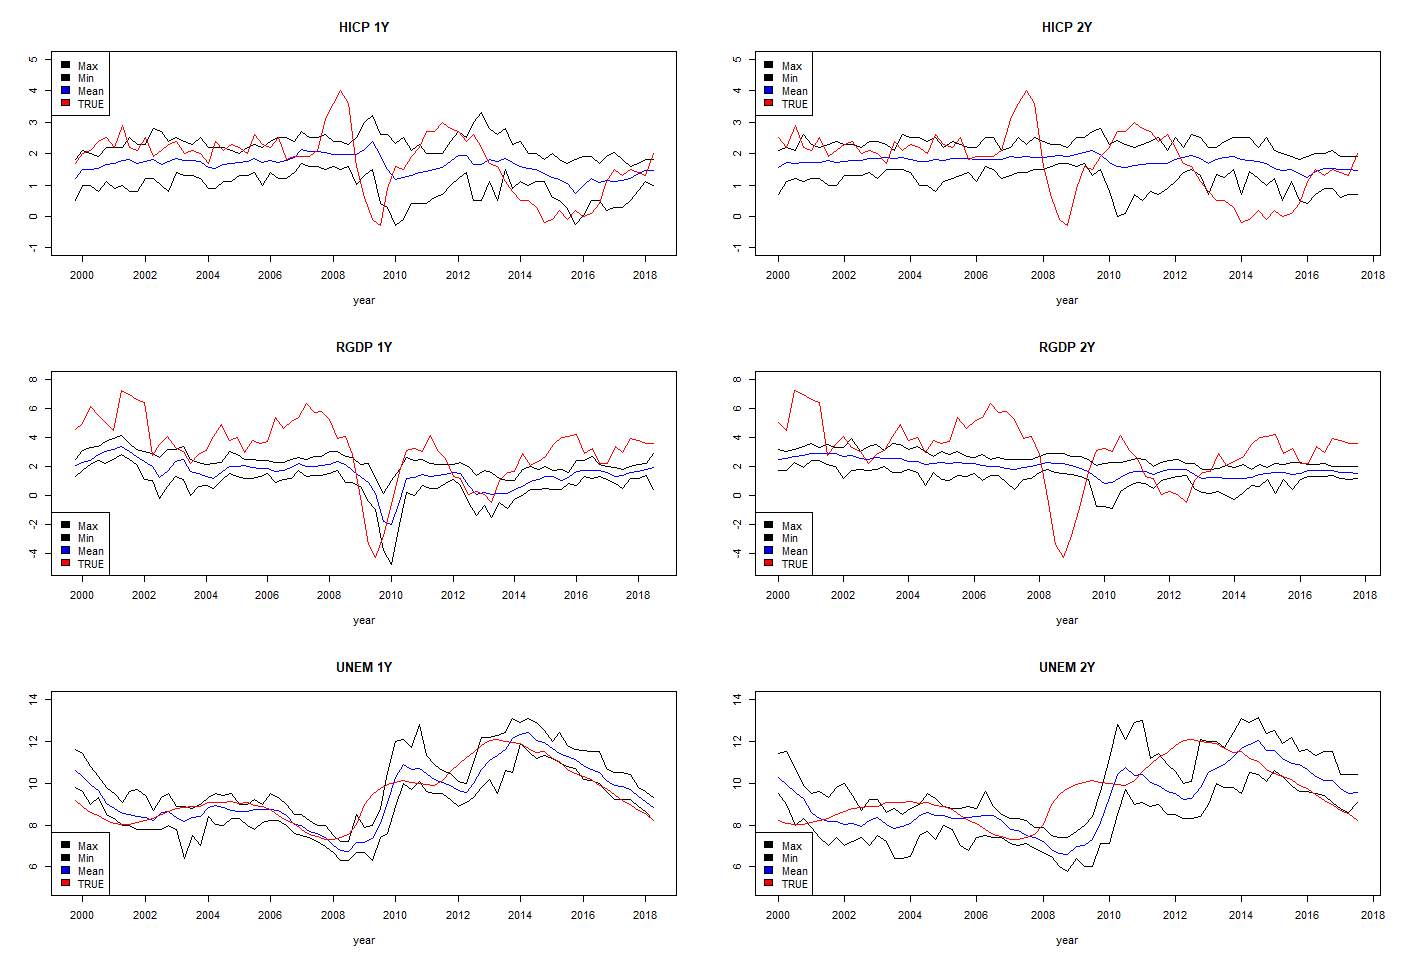
\includegraphics{./Images/SPF.pdf}
	\caption{Survey of Professional Forecasters data illustration}\label{fig: SPF data illustration}
\end{figure}

In figure \ref{fig: SPF data illustration} and table \ref{tab: correlation summary statistics} show the plots of the forecasts alongside with the true value in the macroeconomics and the statistics of the covariance of the forecast error. We plot only the minimum, mean, and maximum from the forecasts. We see that there exist a high consistency across all forecasts, with two years ahead stronger than one year. The consistency in the forecast is lower in UNEM than the other two. Furthermore, many true values lie outside of the forecast range, with RGDP the worse of all three. More values outside of the forecast range suggest that restricting positive weight may be a strong limitation in the forecast combination.

We examine the amount of true value outside of the forecast range by looking at the summary statistics. Let model space be an indicator with 1 when the true value is outside of the forecast range, and 0 when the true value is inside. Table \ref{tab: modelspace summary statistics} shows the mean of the indicator. From the three macro topics, RGDP has the highest percentage of time periods to be outside the forecast range, 83\%, followed by HICP with an average of 48\% of the time periods. UNEM with 38\% of the time periods has the lowest percentage to be outside the forecast range. Changing from one year to two years generally does not influence the mean of the indicator a lot. From the results from figure \ref{fig: SPF data illustration} and table \ref{tab: modelspace summary statistics}, we expect to have large effect using truncation in the forecast of RGDP, while HICP and UNEM do not have a strong effect. We also expect the two years ahead forecast will be better than the one year ahead.

\begin{table}[!h]
	\centering
	\caption{Mean of the model space indicator of the forecast. The indicators are split up into different forecast topics and different forecast horizons. From the three macro topics, RGDP has the least chance within the forecast range, followed by HICP. UNEM has the highest chance to be in the forecast range.}
	\label{tab: modelspace summary statistics}
	\begin{tabular}{lcccccc}
		\hline
		&\multicolumn{6}{c}{Model Space Indicator}\\
		\cmidrule(lr){2-7}
		Macro topic & \multicolumn{2}{c}{HICP} & \multicolumn{2}{c}{RGDP} & \multicolumn{2}{c}{UNEM} \\
		\cmidrule(lr){2-3} \cmidrule(lr){4-5}\cmidrule(lr){6-7}
		Horizon     & one year & two years & one year & two years & one year & two years \\ 
		\hline
		Mean        & 0.45        & 0.51         & 0.83        & 0.82        & 0.37         & 0.39       \\
		\hline
	\end{tabular}
\end{table}

As not all forecasters replied to each survey, we show the number of forecasters per macroeconomic topic in table \ref{tab: amount of forecasters}. The amount of forecasters after filtering is around 70 for one year ahead forecasts, and 60 for two years ahead forecasts. We also show the number of replies per forecaster in a summary statistic in table \ref{tab: forecaster summary statistics}. The minimum amount of forecast is set to 24, and all forecasters with less than 24 forecasts are discarded. The maximum replies are around 70, which is close to the full amount of 75 observations. With the mean around 50, we have enough observations to do pair-wise covariance, but multivariate covariance remains sceptical.

\begin{table}[!h]
	\centering
	\caption{Amount of Forecasters. The amount of forecasters for one year ahead forecast is higher than two years ahead.}
	\label{tab: amount of forecasters}
	\begin{tabular}{lcccccc}
		\hline
		&\multicolumn{6}{c}{Amount of Forecasters}\\
		\cmidrule(lr){2-7}
		Macro topic & \multicolumn{2}{c}{HICP} & \multicolumn{2}{c}{RGDP} & \multicolumn{2}{c}{UNEM} \\
		\cmidrule(lr){2-3} \cmidrule(lr){4-5}\cmidrule(lr){6-7}
		Horizon     & one year & two years & one year & two years & one year & two years \\ 
		\hline
		Amount        &      72   &60          &70         &64         & 65         & 53       \\
		\hline
	\end{tabular}
\end{table}

\begin{table}[!h]
	\centering
	\caption{Summary statistics of the survey reply amounts per forecasters. The average forecasters made around 50 replies for the whole duration of the survey. No forecaster replied to all survey. Means are round down to whole numbers for readability.}
	\label{tab: forecaster summary statistics}
	\begin{tabular}{lcccccc}%{S[table-format=3.2]}
		\hline
		&\multicolumn{6}{c}{Summary Statistics of the Amounts Per Forecaster}\\
		\cmidrule(lr){2-7}
		Macro topic & \multicolumn{2}{c}{HICP} & \multicolumn{2}{c}{RGDP} & \multicolumn{2}{c}{UNEM} \\
		\cmidrule(lr){2-3} \cmidrule(lr){4-5}\cmidrule(lr){6-7}
		Horizon     & one year & two years & one year & two years & one year & two years \\ 
		\hline
		Minimum & 24    & 24    & 26    & 24    & 25    & 24    \\
		First Q & 40    & 40    & 42    & 35    & 40    & 36    \\
		Median  & 55    & 52    & 55    & 51    & 53    & 52    \\
		Mean    & 53    & 50    & 54    & 49    & 52    & 50    \\
		Third Q & 67    & 62    & 66    & 63    & 66    & 63    \\
		Maximum & 74    & 70    & 75    & 71    & 74    & 70      \\ 
		\hline
	\end{tabular}
\end{table}

Table \ref{tab: time summary statistics} shows the summary statistics of the number of survey replies per time period. On average there are 40 replies per time period. The deviation to the time is small with more than 50\% within 35 to 45 range. The minimum of 22 in UNEM pose a possible problem in the estimation of the covariance. If the estimation of the covariance is bad, limiting negative weights will pose a better result.

\begin{table}[!h]
	\centering
	\caption{Summary statistics of the survey reply amount per time period. There are around 35 to 45 responses for half of the time. Means are round down to whole numbers for readability.}
	\label{tab: time summary statistics}
	\begin{tabular}{lcccccc}%{S[table-format=3.2]}
		\hline
		&\multicolumn{6}{c}{Summary Statistics of the Amounts Per Time Period}\\
		\cmidrule(lr){2-7}
		Macro topic & \multicolumn{2}{c}{HICP} & \multicolumn{2}{c}{RGDP} & \multicolumn{2}{c}{UNEM} \\
		\cmidrule(lr){2-3} \cmidrule(lr){4-5}\cmidrule(lr){6-7}
		Horizon     & one year & two years & one year & two years & one year & two years \\ 
		\hline
		Minimum & 37    & 26    & 38    & 28    & 32    & 22    \\
		First Q & 43    & 35    & 42    & 36    & 38    & 30    \\
		Median  & 45    & 38    & 45    & 40    & 40    & 34    \\
		Mean    & 46    & 39    & 45    & 40    & 41    & 34    \\
		Third Q & 49    & 43    & 48    & 45    & 44    & 38    \\
		Maximum & 54    & 49    & 54    & 52    & 51    & 44       \\ 
		\hline
	\end{tabular}
\end{table}

Table \ref{tab: amount per test period} shows the number of replies per time period that we use to test the model. The values are lower than the mean for almost all time period except a few. Only RGDP one year on 2018 Q1 and 2018 Q2 and UNEM one year on 2016Q1 are above the average. The low number decreases the dimension of the covariance matrix, but on the other hand, decreases the number of observations. The trade-off between lower dimension should be more important than the loss in observations.

\begin{table}[!h]
	\centering
	\caption{Amount of replies to the survey on the testing period starting 2016. All forecasters that replied in the test periods had also replied in previous time periods.}
	\label{tab: amount per test period}
	\begin{tabular}{lcccccc}%{S[table-format=3.2]}
		\hline
		&\multicolumn{6}{c}{Survey Reply Amounts}\\
		\cmidrule(lr){2-7}
		Macro topic & \multicolumn{2}{c}{HICP} & \multicolumn{2}{c}{RGDP} & \multicolumn{2}{c}{UNEM} \\
		\cmidrule(lr){2-3} \cmidrule(lr){4-5}\cmidrule(lr){6-7}
		Test Period     & one year & two years & one year & two years & one year & two years \\ 
		\hline
		2016 Q1      & 45    & 32    & 38    & 33    & 41    & 30    \\
		2016 Q2      & 40    & 33    & 42    & 37    & 36    & 28    \\
		2016 Q3      & 44    & 35    & 42    & 38    & 39    & 28    \\
		2016 Q4      & 45    & 34    & 41    & 40    & 39    & 30    \\
		2017 Q1      & 39    & 35    & 38    & 30    & 32    & 32    \\
		2017 Q2      & 38    & 27    & 38    & 35    & 33    & 25    \\
		2017 Q3      & 37    & 31    & 43    & 36    & 33    & 29    \\
		2017 Q4      & 43    & 34    & 41    & 36    & 36    & 29    \\
		2018 Q1      & 40    & 27    & 46    & 30    & 34    & 22    \\
		2018 Q2      & 44    & 26    & 45    & 31    & 40    & 23    \\ 
		\hline
	\end{tabular}
\end{table}

The table \ref{tab: correlation summary statistics} tell us on how the forecast errors are correlated. The correlations are split up into different forecast topics and different forecast horizons. The diagonal elements of the correlation matrix are not within the table when generating the summary statistics. For all of the series, the correlations are on average above 60\%. In HICP and UNEM the correlation increases across all statistics when the forecast horizon increases, while RGDP remains the same. The lowest correlation to be found is -0.02, but this number is not too different from the minimum correlation in the other two topics.

\begin{table}[!h]
	\centering
	\caption{Summary statistics of the correlation of the forecast error. The correlations are split up into different forecast topics and different forecast horizons. For all of the series, the correlations are on average above 60\%. In HICP and UNEM the correlation increases across all statistics when the forecast horizon increases, while RGDP remains the same.}
	\label{tab: correlation summary statistics}
	\begin{tabular}{lcccccc}%{S[table-format=3.2]}
		\hline
		&\multicolumn{6}{c}{Correlation}\\
		\cmidrule(lr){2-7}
		Macro topic & \multicolumn{2}{c}{HICP} & \multicolumn{2}{c}{RGDP} & \multicolumn{2}{c}{UNEM} \\
		\cmidrule(lr){2-3} \cmidrule(lr){4-5}\cmidrule(lr){6-7}
		Horizon     & one year & two years & one year & two years & one year & two years \\ 
		\hline
		Minimum     & 0.03        & 0.02        & 0.11        & 0.13        & -0.02        & 0.08       \\
		First Q     & 0.53        & 0.62        & 0.63        & 0.65        & 0.47         & 0.56       \\
		Mean        & 0.64        & 0.70        & 0.75        & 0.75        & 0.59         & 0.67       \\
		Median      & 0.66        & 0.72        & 0.81        & 0.80        & 0.62         & 0.70       \\
		Third Q     & 0.77        & 0.81        & 0.89        & 0.87        & 0.74         & 0.80       \\
		Maximum     & 0.96        & 0.97        & 0.98        & 0.98        & 0.94         & 0.95       \\ 
		\hline
	\end{tabular}
\end{table}


We conclude for the analysis of SPF that there exhibit characteristics that are not in the standard cases where correlation are close to 0. By incorporating the possibility of negative weight, we expect to see some improvement in the forecast errors.

\section{Empirical Results}\label{empirical-results}
\subsection{Optimal Weight}\label{optimal-weight}
Analysis of the optimal weight given by equation \ref{eqn: simple weight} provides us with a preliminary understanding of the variability. Table \ref{tab: simple weight summary statistics} shows the summary statistics of the optimal weight. We see that for all macroeconomic topics, the mean and median variate around 0.02, which is close to the calculation from equal weight. Looking at the first and the third quantile, we see that half of the weight are between -0.6 and 0.6, which gives us a possible range of effectiveness of the threshold. The minimum and the maximum is extreme considering that 1 is 100\%. With negativity up to -11, -21, and -14, and first and third quartile only up to -0.6 and 0.6, the weight indicates a strong thick tail behaviour. In the difference between one year and two years ahead, for two out of three macro topics, the extreme values converge to 0. RGDP becomes worse. On the other hand, the gap between the first and the third quantile increases for all topics. This indicates the increase in the choice of negative weight in the general cases for two years horizon. The mean and median does not change much in relation to the forecast horizon.

\begin{table}[!h]
	\centering
	\caption{Summary statistics of the weight from equation \ref{eqn: simple weight}. The mean and median is close to the value from equal weight. However, extreme values exist in the weight, visible in the minimum and maximum. Based on the first and the third quantile, we see that half of the weight are between -0.6 and 0.6.}
	\label{tab: simple weight summary statistics}
	\begin{tabular}{lcccccc}%{S[table-format=3.2]}
		\hline
		&\multicolumn{5}{c}{Optimal Weight}\\
		\cmidrule(lr){2-7}
		Macro topic & \multicolumn{2}{c}{HICP} & \multicolumn{2}{c}{RGDP} & \multicolumn{2}{c}{UNEM} \\
		\cmidrule(lr){2-3} \cmidrule(lr){4-5}\cmidrule(lr){6-7}
		Horizon     & one year & two years & one year & two years & one year & two years \\ 
		\hline
		Minimum      & -11.05      & -6.21      & -9.00      & -21.79      & -14.41      & -5.64      \\
		First Q      & -0.30       & -0.59      & -0.20      & -0.63       & -0.28       & -0.40      \\
		Mean         & 0.04        & 0.04       & 0.01       & -0.01       & 0.03        & 0.05       \\
		Median       & 0.05        & 0.03       & 0.04       & 0.01        & 0.04        & 0.03       \\
		Third Q      & 0.41        & 0.60       & 0.25       & 0.82        & 0.39        & 0.43       \\
		Maximum      & 12.94       & 7.56       & 8.74       & 16.34       & 11.26       & 7.90       \\ 
		\hline
	\end{tabular}
\end{table}

\subsection{Proceure}\label{proceure}

We seek to evaluate the effect of truncating the weight with SPF data. The procedure to get the weight can be different between different researchers. Therefore we provide an exact order of the steps taken in the weight estimation. The weight estimation for the truncation using the following steps:


Given each time to forecast, we take all the know observation before that forecast time period.

\begin{enumerate}
	\def\labelenumi{\arabic{enumi}.}
	\item
Find the nearest positive definite covariance matrix. This step is required for the covariance to be invertible. We employ the nearPD function from r package \emph{Matrix}. The nearPD function first decomposes the covariance into univariate variance and the correlation. The function then uses the algorithm by \emph{higham} on the correlation matrix to compute the nearest positive definite matrix. The final result is the covariance matrix that is combined from the univariate variance and the correlation matrix.
	\item
Subset the covariance. We take the submatrix containing only the available forecast on the testing period. If 80 forecasters had made some forecasts before, but out of them, only 40 has a forecast this time, we discard the 40 extra forecasters.
	\item
Estimate the optimal weight \(w^*\) from equation
	\ref{eqn: simple weight}.
	\item
	Truncate the optimal weight with equation \ref{eqn: w trunc}. The weight now has fewer values and does not sum to one. We normalise the weights back such that the sum of the weights is 1.
	\item
	Combine the forecast using the new weights.
	\item
	Calculate the test statistics of new weights and equal weights.
	\item
	Calculate the ratio of the test statistics of new weights over equal weights.
\end{enumerate}

\subsection{Ratio of Test Statistics}\label{ratio-of-test-statistics}
The ratio of test statistics is best determined by evaluating the performance of various weights using mean absolute prediction error (MAPE) and mean squared prediction error (MSPE). The comparison is made between MSPE and the truncated MAPE and MSPE from the same weight to come up with a test ratio. Results of UNEM, RGDP and HICP are then documented, and the ratio of the MAPE and MSPE are reported to assist in the visualising the impact of truncation rather than comparing per number to the same weights. The test statistic of the truncation is considered to be smaller than the test statistic with the same weight if the value is less than 1. The weights below the threshold $c$ are set to $c$.

From table \ref{tab: c MSPE HICP}, it is clear that with truncation values -0.5 and -1.5, the MSPE is obtained for one year horizon and two years horizon respectively. In that same regard, the minimum of MAPE is attained at -1 and -1.5 respectively. The corresponding two years choice or selection that is based on the MAPE is seen to have collided with the selection that has been made based on the MSPE. Furthermore, the -1.5 is the only threshold with a ratio lower than 1 for MAPE two years horizon. The ratio in MSPE differs largely from 1, with 0.91 and 0.93 for 1 and 2 years. This effect is not visible in MAPE ratio.

\begin{table}[!h]
	\centering
	\caption{Mean Squared Prediction Error (MSPE) and Mean Absolute Prediction Error (MAPE) of inflation with different truncated value. The MSPE and MAPE of the truncated value are given in the ratio of truncation to equal weight. Larger than 1 means truncated is worse, whereas smaller than 1 means truncated weight helps in reducing MSPE or MAPE.}
	\label{tab: c MSPE HICP}
	\begin{tabular}{lcccc}
		\hline\hline
		&                        \multicolumn{4}{c}{HICP}                         \\
		\cmidrule(lr){2-5}                              & \multicolumn{2}{c}{one year Horizon} & \multicolumn{2}{c}{two years Horizon} \\
		\cmidrule(lr){2-3} \cmidrule(lr){4-5}
		Threshold & MSPE Ratio &    MAPE Ratio    & MSPE Ratio &    MAPE Ratio    \\ \hline
-$\infty$ & 3.2902 & 1.5898 & 2.2072 & 1.4347\\ 
-5 & 2.8209 & 1.4174 & 2.0871 & 1.3563\\ 
-4.5 & 2.8209 & 1.4175 & 2.0296 & 1.2925\\ 
-4 & 2.8208 & 1.4173 & 2.0475 & 1.3145\\ 
-3.5 & 2.8203 & 1.4166 & 1.8539 & 1.268\\ 
-3 & 2.8196 & 1.4156 & 1.6821 & 1.212\\ 
-2.5 & 2.8191 & 1.4147 & 1.2439 & 1.1119\\ 
-2 & 2.0779 & 1.2606 & 1.0318 & 1.0604\\ 
-1.5 & 1.1934 & 1.0686 & 0.925 & 0.9852\\ 
-1 & 0.9389 & 0.9819 & 0.9587 & 1.029\\ 
-0.5 & 0.9101 & 0.9875 & 0.9724 & 1.0201\\ 
0 & 0.9844 & 0.9994 & 0.9834 & 1.0005\\ 
\hline\hline
	\end{tabular}
\end{table}

RGDP is reported in table \ref{tab: c MSPE RGDP}.  The one year threshold is approximately -1 and -1.5 thereby obtaining 0.83 and 0.89 for MSPE and MAPE respectively. On a two years horizon, the MAPE the MAPE behaves differently. MSPE for RGDP two years did not reach the minimum in the range of -5 to 0. We did not search further below -5 for the minimum. A boundary case that is realized because of this cut-off is 1.01. The least MAPE is observed to be attended at -4.5 with a ratio of 0.91. In one year horizon, the optimal weight MSPE ratio has a score of 1.44 showing that it was similar to equal weight. With a ratio of 6.07, on the other hand, two years horizon does not seem to perform so well in optimal weight. For two and one year, the optimal MAPE ratio shows that there are similar values of 1.80 and 1.07 respectively to equal weights.

\begin{table}[!h]
	\centering
	\caption{Mean Squared Prediction Error (MSPE) and Mean Absolute Prediction Error (MAPE) of economic growth with different truncated value. The MSPE and MAPE of the truncated value are given in the ratio of truncation to equal weight. Larger than 1 means truncated is worse, whereas smaller than 1 means truncated weight helps in reducing MSPE or MAPE.}
	\label{tab: c MSPE RGDP}
	\begin{tabular}{lcccc}
		\hline\hline
		&                        \multicolumn{4}{c}{RGDP}                         \\
		\cmidrule(lr){2-5}                              & \multicolumn{2}{c}{one year Horizon} & \multicolumn{2}{c}{two years Horizon} \\
		\cmidrule(lr){2-3} \cmidrule(lr){4-5}
		Threshold & MSPE Ratio &    MAPE Ratio    & MSPE Ratio &    MAPE Ratio    \\ \hline
-$\infty$ & 1.4387 & 1.0681 & 6.0654 & 1.8047\\ 
-5 & 1.0854 & 0.944 & 1.0474 & 0.9234\\ 
-4.5 & 1.0911 & 0.9491 & 1.0385 & 0.9087\\ 
-4 & 1.1081 & 0.9622 & 1.0445 & 0.9277\\ 
-3.5 & 1.1021 & 0.9657 & 1.0537 & 0.9401\\ 
-3 & 0.9826 & 0.9389 & 1.0571 & 0.9462\\ 
-2.5 & 0.9076 & 0.9164 & 1.0663 & 0.9604\\ 
-2 & 0.8654 & 0.8987 & 1.0722 & 0.9677\\ 
-1.5 & 0.8408 & 0.8856 & 1.0847 & 0.977\\ 
-1 & 0.8309 & 0.8894 & 1.1191 & 1.0273\\ 
-0.5 & 0.8523 & 0.9125 & 1.047 & 1.0219\\ 
0 & 0.9721 & 0.9844 & 1.0073 & 1.0056\\ 
		\hline\hline
	\end{tabular}
\end{table}

If we take a close look at UNEM, the results that have been provided tend to give ratios that are promising. The lowest MSPE ratio was registered by UNEM for one year and two years at -1 and 0 respectively. As before, we do not search beyond 0 in this thesis. Comparing to HICP and RGDP, the MSPE ratio of 0.60 and 0.83 are the lowest of all three.  Moreover, a 0.73 MAPE one year ratio and 0.90 two years ratio at -1.5 and -0.5 shows positive news. Interesting to note is the optimal weight in MAPE one year is already 0.89. This is lower than the other macroeconomic topics.

\begin{table}[!h]
	\centering
	\caption{Mean Squared Prediction Error (MSPE) and Mean Absolute Prediction Error (MAPE) of unemployment with different truncated value. The MSPE and MAPE of the truncated value are given in the ratio of truncation to equal weight. Larger than 1 means truncated is worse, whereas smaller than 1 means truncated weight helps in reducing MSPE or MAPE.}
	\label{tab: c MSPE UNEM}
	\begin{tabular}{lcccc}
		\hline\hline
		&                        \multicolumn{4}{c}{UNEM}                         \\
		\cmidrule(lr){2-5}                              & \multicolumn{2}{c}{one year Horizon} & \multicolumn{2}{c}{two years Horizon} \\
		\cmidrule(lr){2-3} \cmidrule(lr){4-5}
		Threshold & MSPE Ratio &    MAPE Ratio    & MSPE Ratio &    MAPE Ratio    \\ \hline
-$\infty$ & 1.1639 & 0.8899 & 4.3535 & 1.6517\\ 
-5 & 1.0247 & 0.8437 & 3.1368 & 1.5265\\ 
-4.5 & 0.863 & 0.7843 & 2.8128 & 1.481\\ 
-4 & 0.8159 & 0.7345 & 2.5409 & 1.4332\\ 
-3.5 & 0.8384 & 0.7679 & 2.3461 & 1.3901\\ 
-3 & 0.8718 & 0.7893 & 2.1681 & 1.332\\ 
-2.5 & 0.8885 & 0.7972 & 2.0443 & 1.2694\\ 
-2 & 0.8206 & 0.7977 & 1.9581 & 1.2442\\ 
-1.5 & 0.6761 & 0.7379 & 1.8529 & 1.2262\\ 
-1 & 0.6033 & 0.6819 & 1.55 & 1.0992\\ 
-0.5 & 0.6454 & 0.725 & 1.0037 & 0.933\\ 
0 & 0.9346 & 0.9543 & 0.8769 & 0.9466\\ 
		\hline\hline
	\end{tabular}
\end{table}

From figure \ref{fig: c Ratio sub} plotted using a 0.1 step size, HICP inhibits a relatively quick reduction in both minor changes and statistics thereafter. RGDP shows an increase in the lower threshold for one year and a U-shape afterwards. RGDP two years has an odd behaviour showing first a U-shape around -4.5 and then a drop after -1. UNEM one year shows an error of a W-shape. This shows that the changes in variance reduction and/or bias increment are not gradual, causing the step-like look of the test statistics. UNEM two years, on the other hand, impose a clean slope downwards.

\begin{figure}[!h]
	\centering
	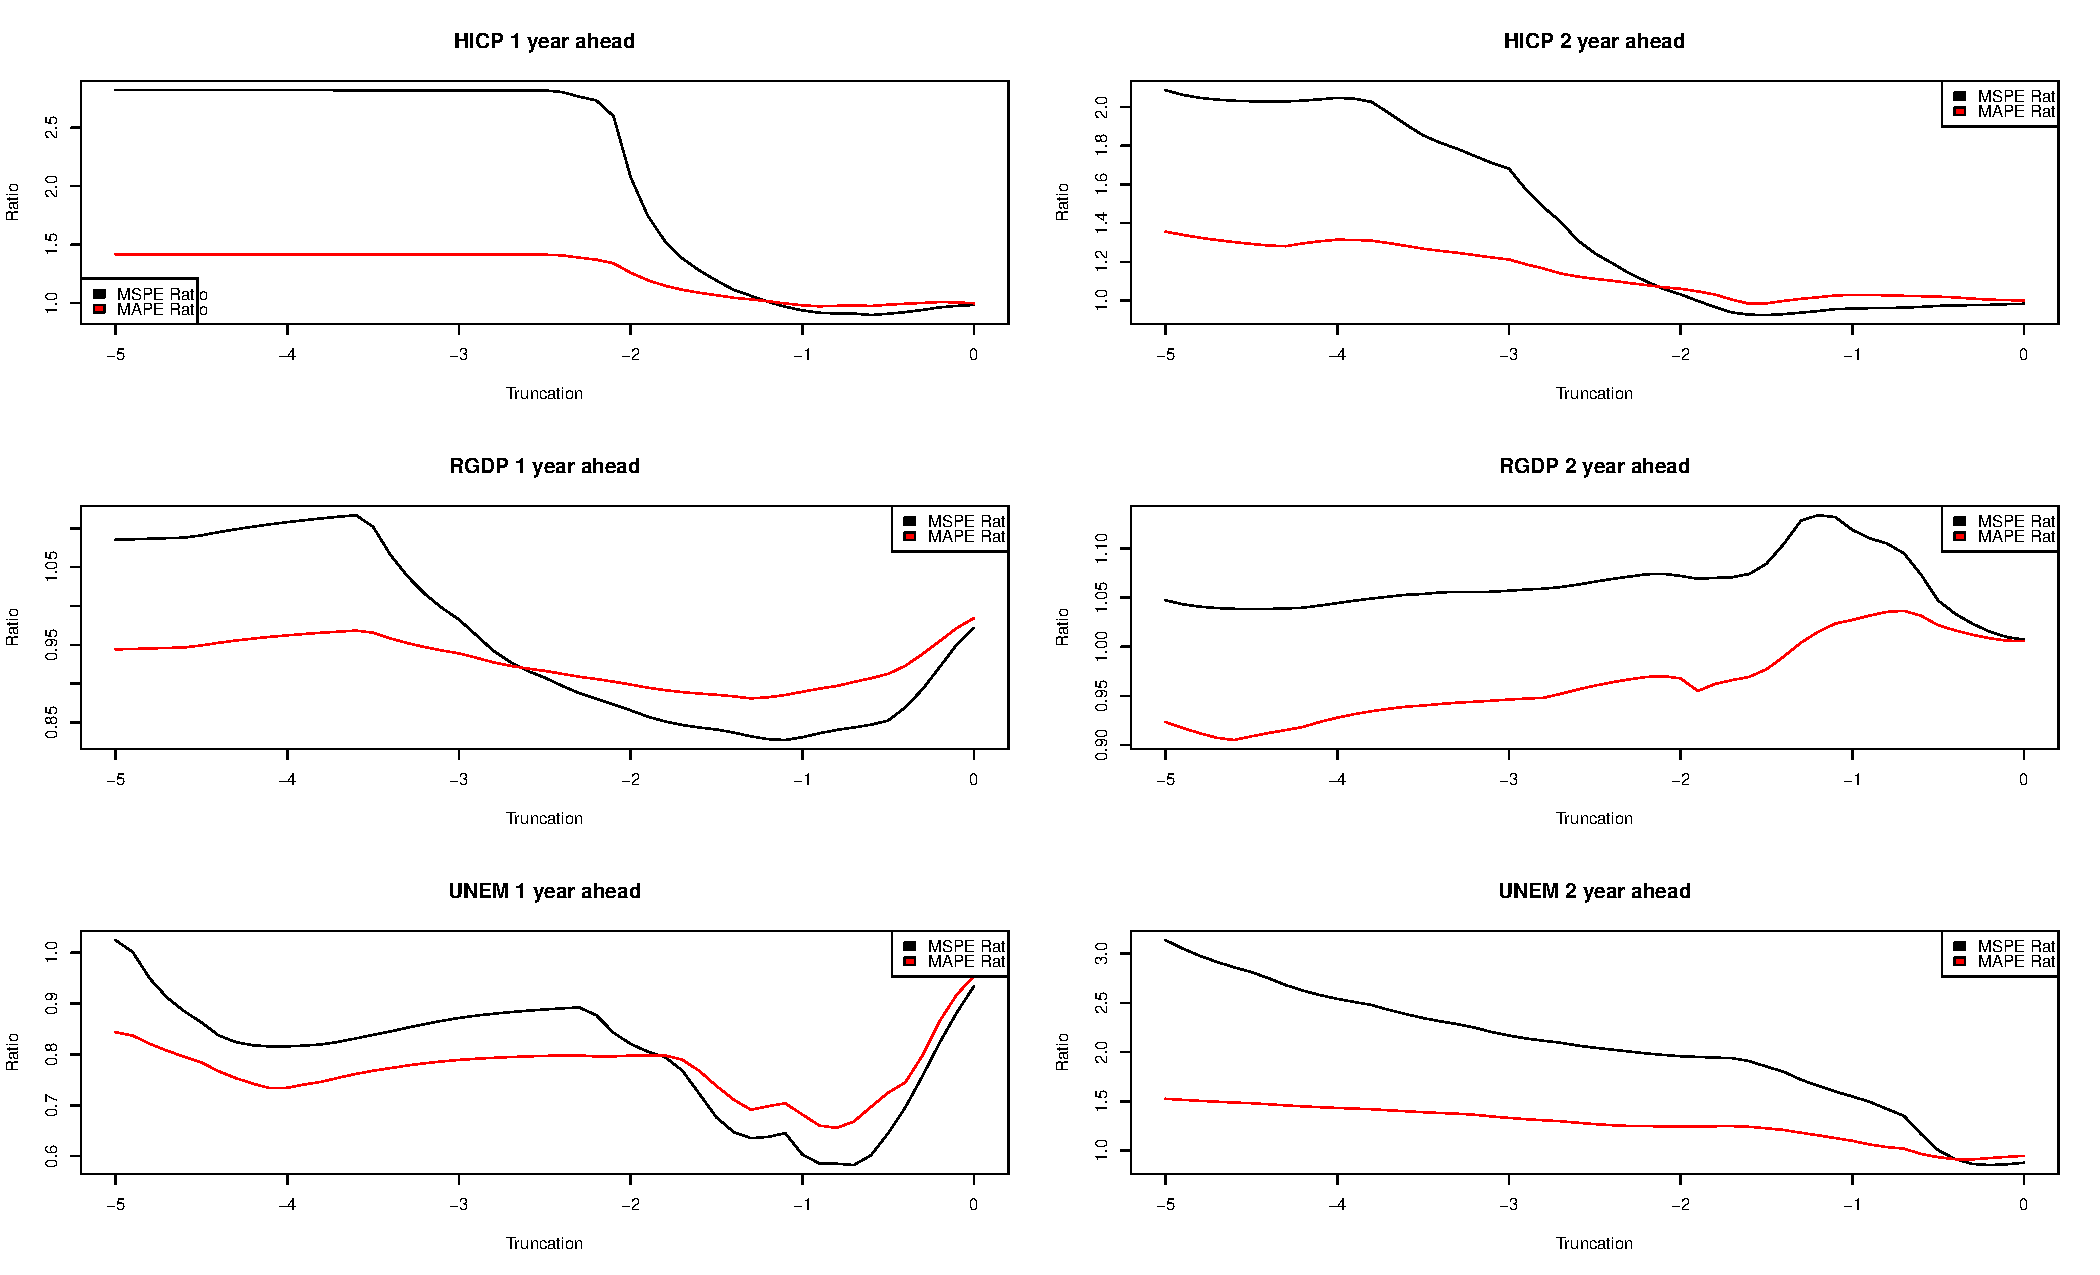
\includegraphics{./Images/Ratio_c.pdf}
	\caption{MSPE Ratio for different macroeconomic topics}\label{fig: c Ratio sub}
\end{figure}

This section shows that it is possible to outperform equal weights and no negative weights under certain circumstances. Five out of six macroeconomic topics show positive news. This is promising as we show that there is no need to go full in.

\subsection{Ratio with $c$ as $0$}\label{ratio-of-mean-squared-prediction-error}
Section \ref{ratio-of-test-statistics} shows the effect of truncation. This section looks at a special case of the truncation. The weights that are below the threshold are set to $0$. In other words, doing so effectively removes the forecast. This is an interesting case due to the intersection between threshold and variable selection. The difference in section \ref{ratio-of-test-statistics} and section \ref{ratio-of-mean-squared-prediction-error} can then partially be explained by the difference in forecast combination and forecast selection.

We see in table \ref{tab: MSPE HICP} that for the truncation value -2 and -1.5, the minimum of MSPE is attained for one year horizon and two years horizon respectively. The minimum of MAPE are attended at -2 and 0 respectively. The one year selection based on MAPE collides with selection based on MSPE, but the minimum for MAPE is not at -1.5. The optimal weight obtains a ratio of 3.29 and 2.21 for MSPE, significantly larger than the ratio obtained by truncation. The ratio difference of MAPE between optimal weight and truncated weights are smaller compared with MSPE. Truncating all the way to 0 means that no forecast with weight less than 0 is selected. For HICP, selecting too strict threshold does not help in 3 out of 4 cases.


\begin{table}[!h]
	\centering
	\caption{Mean Squared Prediction Error (MSPE) and Mean Absolute Prediction Error (MAPE) of inflation with the truncated value set to 0. The MSPE and MAPE of the truncated value are given in the ratio of truncation to equal weight. Larger than 1 means truncated is worse, whereas smaller than 1 means truncated weight helps in reducing MSPE or MAPE.}
	\label{tab: MSPE HICP}
	\begin{tabular}{lcccc}
		\hline\hline
		&                        \multicolumn{4}{c}{HICP}                         \\
		\cmidrule(lr){2-5}                              & \multicolumn{2}{c}{one year Horizon} & \multicolumn{2}{c}{two years Horizon} \\
		\cmidrule(lr){2-3} \cmidrule(lr){4-5}
		Threshold & MSPE Ratio &    MAPE Ratio    & MSPE Ratio &    MAPE Ratio    \\ \hline
		-$\infty$ & 3.2902 & 1.5898 & 2.2072 & 1.4347\\ 
		-5 & 2.8211 & 1.4178 & 2.1148 & 1.3537\\ 
		-4.5 & 2.8211 & 1.4178 & 2.1148 & 1.3537\\ 
		-4 & 2.8187 & 1.414 & 2.1500 & 1.3753\\ 
		-3.5 & 2.8178 & 1.4126 & 1.6747 & 1.1988\\ 
		-3 & 2.8178 & 1.4126 & 1.5479 & 1.1551\\ 
		-2.5 & 2.8180 & 1.4129 & 1.0181 & 1.0638\\ 
		-2 & 0.8078 & 0.9025 & 0.993 & 1.0653\\ 
		-1.5 & 0.8877 & 0.9619 & 0.9688 & 1.0390\\ 
		-1 & 0.8835 & 0.9610 & 0.9764 & 1.0170\\ 
		-0.5 & 0.9465 & 0.9912 & 0.9877 & 1.0108\\ 
		0 & 0.9844 & 0.9994 & 0.9834 & 1.0005\\ 		 \hline\hline
	\end{tabular}
\end{table}

Table \ref{tab: MSPE RGDP} shows a similar pattern in RGDP as in HICP. The optimal threshold for one year is around -1.5, obtaining 0.83 and 0.88 for MSPE and MAPE respectively. We did not look for a threshold larger than 0, and the minimum MSPE of RGDP two years is not within the search region. This cut-off gives us 1.01 as the boundary case. The MAPE on two years horizon acts differently. The minimum MAPE is attended at -4.5. The optimal weight MSPE ratio in one year horizon is similar to equal weight, scoring 1.44 in the ratio. Two years ahead MSPE ratio, on the other hand, does not perform that well in optimal weight, with a ratio of 6.07. The optimal weight in MAPE ratio for one and two years show similar values to equal weights, scoring 1.07 and 1.80 respectively.

\begin{table}[!h]
	\centering
	\caption{Mean Squared Prediction Error (MSPE) and Mean Absolute Prediction Error (MAPE) of economic growth with the truncated value set to 0. The MSPE and MAPE of the truncated value are given in the ratio of truncation to equal weight. Larger than 1 means truncated is worse, whereas smaller than 1 means truncated weight helps in reducing MSPE or MAPE.}
	\label{tab: MSPE RGDP}
	\begin{tabular}{lcccc}
		\hline\hline
		& \multicolumn{4}{c}{RGDP}                                                \\
		\cmidrule(lr){2-5}
		& \multicolumn{2}{c}{one year Horizon} & \multicolumn{2}{c}{two years Horizon} \\
		\cmidrule(lr){2-3} \cmidrule(lr){4-5}
		Threshold & MSPE Ratio &    MAPE Ratio    & MSPE Ratio &    MAPE Ratio    \\ 
		\hline
		-$\infty$ & 1.4387 & 1.0681 & 6.0654 & 1.8047\\ 
		-5 & 1.1000 & 0.9561 & 1.0684 & 0.9496\\ 
		-4.5 & 1.1462 & 0.9861 & 1.0683 & 0.9496\\ 
		-4 & 1.1462 & 0.9861 & 1.0885 & 0.9621\\ 
		-3.5 & 0.8738 & 0.9029 & 1.0765 & 0.9539\\ 
		-3 & 0.8768 & 0.9046 & 1.0824 & 0.9579\\ 
		-2.5 & 0.8611 & 0.8967 & 1.102 & 0.9899\\ 
		-2 & 0.8402 & 0.8824 & 1.0824 & 0.9567\\ 
		-1.5 & 0.8278 & 0.8768 & 1.1712 & 1.0438\\ 
		-1 & 0.8610 & 0.9102 & 1.1356 & 1.0617\\ 
		-0.5 & 0.8999 & 0.9396 & 1.0198 & 1.0114\\ 
		0 & 0.9721 & 0.9844 & 1.0073 & 1.0056\\  \hline\hline
	\end{tabular}
\end{table}


When we look further in UNEM, the results show well-performing ratios. UNEM achieved the lowest MSPE ratio in one year and two years at -1.5 and -0.5. Comparing to HICP and RGDP, the MSPE ratio of 0.70 and 0.82 are the lowest of all three. The MSPE ratio of 0.70 is also a 40\% decrease in the MSPE, even when the non-truncated is already at 1.16. MAPE ratio shows that in one year ahead, optimal weight already outperforms equal weights with 0.89, but with truncation, the MAPE ratio drops to 0.74. The MAPE ratio in two years ahead decreases to 0.91. UNEM seems to have an effect from truncation that is not explained by the correlation. UNEM does not have a difference in correlation to other macroeconomics topics that cannot be explained by estimation noise. One possible explanation is the optimal choice of the truncation is more consistent and does not vary over time. We evaluate the consistency of the truncation in the out-of-sample selection area.

\begin{table}[!h] 
	\centering
	\caption{Mean Squared Prediction Error (MSPE) and Mean Absolute Prediction Error (MAPE) of unemployment with the truncated value set to 0. The MSPE and MAPE of the truncated value are given in the ratio of truncation to equal weight. Larger than 1 means truncated is worse, whereas smaller than 1 means truncated weight helps in reducing MSPE or MAPE.}
	\label{tab: MSPE UNEM}
	\begin{tabular}{lcccc}
		\hline\hline
		& \multicolumn{4}{c}{UNEM}                                                \\
		\cmidrule(lr){2-5}
		& \multicolumn{2}{c}{one year Horizon} & \multicolumn{2}{c}{two years Horizon} \\
		\cmidrule(lr){2-3} \cmidrule(lr){4-5}
		Threshold & MSPE Ratio &    MAPE Ratio    & MSPE Ratio &    MAPE Ratio    \\ 
		\hline
		-$\infty$ & 1.1639 & 0.8899 & 4.3535 & 1.6517\\ 
		-5 & 1.0249 & 0.8438 & 2.3189 & 1.3796\\ 
		-4.5 & 0.8926 & 0.7991 & 2.3189 & 1.3796\\ 
		-4 & 0.8926 & 0.7991 & 2.2467 & 1.3552\\ 
		-3.5 & 0.9447 & 0.8189 & 2.0462 & 1.3042\\ 
		-3 & 0.9335 & 0.8137 & 1.9501 & 1.2435\\ 
		-2.5 & 0.9097 & 0.8050 & 1.9146 & 1.2427\\ 
		-2 & 0.7684 & 0.7858 & 1.8718 & 1.2264\\ 
		-1.5 & 0.6988 & 0.7399 & 1.6610 & 1.1328\\ 
		-1 & 0.7283 & 0.7554 & 1.4222 & 1.0346\\ 
		-0.5 & 0.8232 & 0.8471 & 0.8242 & 0.9066\\ 
		0 & 0.9346 & 0.9543 & 0.8769 & 0.9466\\ \hline\hline
	\end{tabular}
\end{table}


Figure \ref{fig: Ratio sub} shows the MSPE ratio and MAPE ratio for HICP, RGDP, and UNEM with forecast horizon 1 and two years. The figures are plotted with a step size of 0.1. From the figure, HICP shows a sudden decrease in both statistics and minor changes afterwards. RGDP one year shows a similar pattern with a larger increase towards the end. For RGDP two years, there is a spike in both statistics around 1.3. Given that the value never falls below 1, we suspect that the correlation does not capture the error well enough, and there might be a better measure to counter the forecast error. UNEM one year is a bit volatile but exhibits a well-defined U-shape. For UNEM two years, the ratios drop in a smooth way to the minimum.

\begin{figure}[!h]
	\centering
	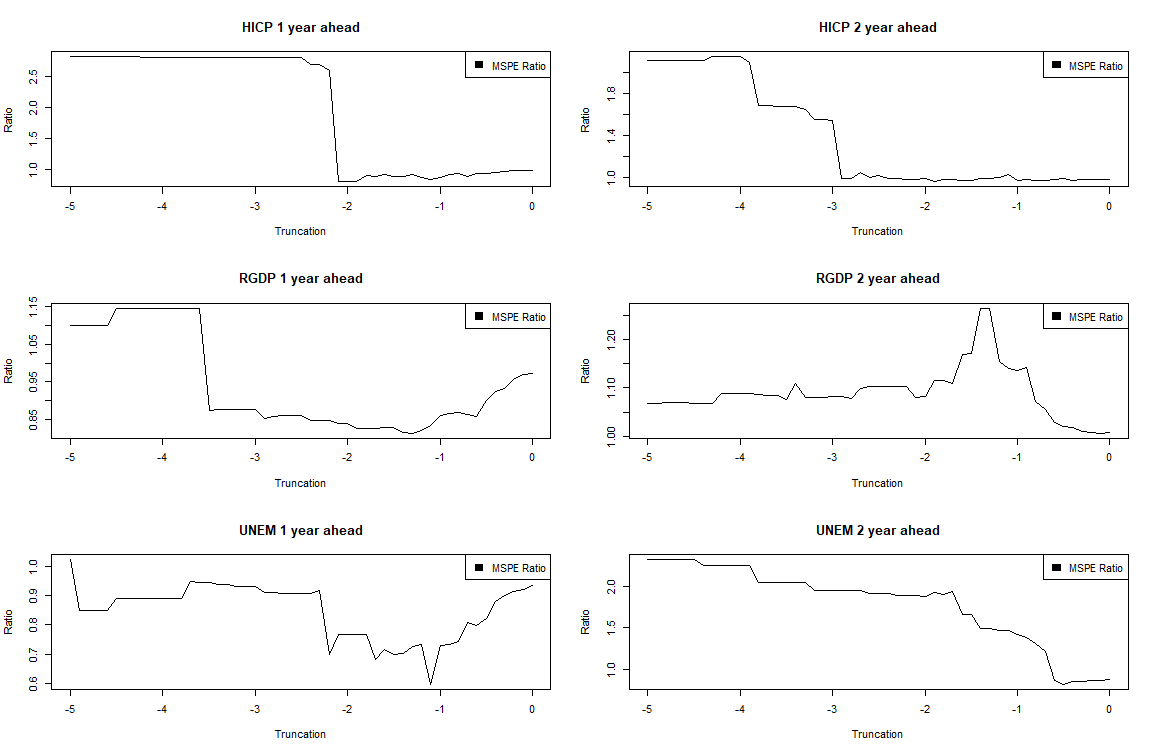
\includegraphics{./Images/Ratio.pdf}
	\caption{MSPE Ratio for different macroeconomic topics}\label{fig: Ratio sub}
\end{figure}

To conclude, we see the possibility to improve the MSPE and MAPE by using the truncation in all cases. In the beginning, there is a drop in the test statistics, but closer to the threshold of 0, test statistics increase. The MSPE and MAPE both have a U-shape characteristic, which attributes to variance and bias. By applying truncation, the drop in variance is larger than the increase in bias, and this contributes to the decrease in the test statistics. It is worth noting that all macroeconomic topics have on an average better performance than equal weight, which is considered a benchmark that is hard to beat. Two of those  macroeconomic forecasts, HICP two years and RGDP 2 year, have a hard to justify the improvement in MSPE or MAPE when estimation error is taken into consideration. Other four obtain from 17\% to 30\% decrease when compared to equal weight. The results also show that the decrease in MSPE is not just one point, but a graduate movement. This implies the robustness in truncation selection. Even if the user does not select the most optimal case, but deviates a small amount next to it, the increase in the test statistics is relatively contained.

\subsection{Optimal Truncation Selection}\label{out-of-sample-truncation-selection}

In this section, we show the MSPE and MAPE in weight truncation when the truncation parameter is in-sample optimally selected. To perform the selection of the truncation parameter, we follow the following step:

\begin{enumerate}
	\def\labelenumi{\arabic{enumi}.}
	\item
	Estimate the optimal weight in equation \ref{eqn: simple weight}.
	\item
	Calculate the in-sample mean squared error (MSE) with truncated weight, e.g., the first window is 1999 Q4 to 2015 Q4. The truncation parameter ranges from -10 to 0 with a step of 0.1. We also look into other starting values, namely -5, -2, and -1.
	\item
	Select the truncation parameter with the lowest in-sample MSE.
	\item
	Use the selected truncation parameter to combine the predictions.
	\item
	Calculate the test statistics of new weights and equal weights.
	\item
	Calculate the ratio of the test statistics of new weights over equal weights.
\end{enumerate}

If there are multiple truncation points with the same MSE value, we take the largest truncation value within the same MSE. The reason to choose the largest value is that the threshold is closer to the next changing point. Assume, for example, a weight with a minimum of -1 is optimal, and any higher weight results in higher MSE. Then all truncation values between -10 and -1 gives the same minimal MSE. We therefore choose -1 to record. The choice does not influence the forecast and is purely for the analysis later.

\subsection{Optimal Truncation Selection Result}\label{out-of-sample-truncation-result}
We evaluate the Optimal Truncation (OT) forecast ability using the same way as section \ref{ratio-of-mean-squared-prediction-error}. The MSPE ratio and the MAPE ratio are given in table \ref{tab: oos mspe}.

As shown in table \ref{tab: oos mspe}, OT improves in all MSPE cases when we compare with equal weights. In MAPE, OT failed to improve HICP one year but obtained positive results in other 5 topics. The truncation works better in RGDP and UNEM. If we compare the value to the MSPE or MAPE of optimal weights, we see that the truncation improves the forecasts for all topics except UNEM one year. RGDP two years also shows in MSPE that none of the constant truncations works as good as changing truncation. This means that the optimal truncation selection overweight the selection uncertainty. These results verify the idea that the truncation improves the upon equal weight even if the truncation uncertainty can increase the MSPE. 

Table \ref{tab: oos mspe} also illustrates the effect of changing the search area. Smaller search area gives less uncertainty but is more restrictive in the solution space. For HICP one year and UNEM 2 year, changing the search area does not influence the test statistics enough to be visible under 4 digits of precision. For HICP two years and RGDP one year, being more restrictive increases the test statistics effectively means worse predictions. For RGDP two years and UNEM one year, being restrictive decreases the prediction error, and therefore MSPE and MAPE. Since being restrictive or not relies on prior information on the forecast set, it is hard to determine which is a good choice.

\begin{table}[!h]
	\centering
	\caption{Mean squared prediction error ratio and mean absolute prediction error ratio when the selection of the truncation is optimal. The minimum search to optimal threshold are -10, -5, -2, and -1.}
	\label{tab: oos mspe}
	\begin{tabular}{lcccccc}
		\hline
		&\multicolumn{6}{c}{MSPE with Optimal Truncation}\\
		\cmidrule(lr){2-7}
		Macro topic & \multicolumn{2}{c}{HICP} & \multicolumn{2}{c}{RGDP} & \multicolumn{2}{c}{UNEM} \\
		\cmidrule(lr){2-3} \cmidrule(lr){4-5}\cmidrule(lr){6-7}
		Threshold     & one year & two years & one year & two years & one year & two years \\ 
		\hline
		-10 & 0.9670   & 0.9611   & 0.9275   & 0.9558   & 0.9153   & 0.8752   \\ 
		-5  & 0.9670   & 0.9611   & 0.9275   & 0.9558   & 0.9153   & 0.8752   \\ 
		-2  & 0.9670   & 0.9719   & 0.9319   & 0.9518   & 0.8982   & 0.8752   \\ 
		-1  & 0.9670   & 0.9709   & 0.9319   & 0.9949   & 0.8982   & 0.8752   \\ 
		\hline
		&\multicolumn{6}{c}{MAPE with Optimal Truncation}\\
		\cmidrule(lr){2-7}
		Macro topic & \multicolumn{2}{c}{HICP} & \multicolumn{2}{c}{RGDP} & \multicolumn{2}{c}{UNEM} \\
		\cmidrule(lr){2-3} \cmidrule(lr){4-5}\cmidrule(lr){6-7}
		Threshold     & one year & two years & one year & two years & one year & two years \\ 
		\hline
		-10 & 1.0015   & 0.9928   & 0.9532   & 0.9577   & 0.9320   & 0.9502   \\
		-5  & 1.0015   & 0.9928   & 0.9532   & 0.9577   & 0.9320   & 0.9502   \\
		-2  & 1.0015   & 0.9968   & 0.9562   & 0.9533   & 0.9260   & 0.9502   \\
		-1  & 1.0015   & 0.9988   & 0.9562   & 0.9524   & 0.9260   & 0.9502   \\
		\hline
	\end{tabular}
\end{table}

To better understand the OT, table \ref{tab: truncation summary statistics} looks at the selection of the truncation. The results show that on average, a truncation around -0.5 is selected, indicating a preference in the negative weight. HICP two years and RGDP two years select on average lower truncation, -0.9 and -1.5 respectively. UNEM selects -0.5 on average, highest among all. The minimum across all macro topics are at most -1, with RGDP one year, RGDP 2 year, and UNEM one year the lowest selected minimum. The first and the third quantiles show that for the most cases, the truncations are not extreme, ranging between -0.5 to -0.2 in one year and -1 to 0 in two years horizon. We notice an increase in the variation when the horizon increases. This can be attributed to the uncertainty in the horizon adds uncertainty in the truncation parameter selection.

\begin{table}[!h]
	\centering
	\caption{Summary statistics of the truncation selected. The available truncation ranges from -10 to 0 with steps of 0.1. Additionally, we add -$\infty$ to the truncation choice, essentially return the non-truncated weight.}
	\label{tab: truncation summary statistics}
	\begin{tabular}{lcccccc}%{S[table-format=3.2]}
		\hline
		&\multicolumn{6}{c}{Selected Optimal Truncation}\\
		\cmidrule(lr){2-7}
		Macro topic & \multicolumn{2}{c}{HICP} & \multicolumn{2}{c}{RGDP} & \multicolumn{2}{c}{UNEM} \\
		\cmidrule(lr){2-3} \cmidrule(lr){4-5}\cmidrule(lr){6-7}
		Horizon     & one year & two years & one year & two years & one year & two years \\ 
		\hline
		Minimum     & -1.3        & -3.8        & -3.4        & -10         & -3.3        & -1.2        \\
		First Q     & -0.7        & -1.0        & -0.5        & -1.1        & -0.4        & -0.3        \\
		Mean        & -0.5        & -0.9        & -0.5        & -1.5        & -0.5        & -0.3        \\
		Median      & -0.4        & -0.6        & -0.3        & -0.4        & -0.3        & -0.3        \\
		Third Q     & -0.4        & -0.4        & -0.1        & -0.2        & -0.2        & 0.0         \\
		Maximum     & 0.0         & 0.0         & 0.0         & 0.0         & -0.1         & 0.0         \\ 
		\hline
	\end{tabular}
\end{table}

Figure \ref{fig: fluctuation} gives a visual inspection on the stability of the selection. For all cases, the fluctuation is limited. Excluding the spikes in some plots, the selection ranges within -1.5 to 0. We suspect that by setting the search range from -1.5 to 0 will improve the OOS truncation selection. 

\begin{figure}[!h]
	\centering
	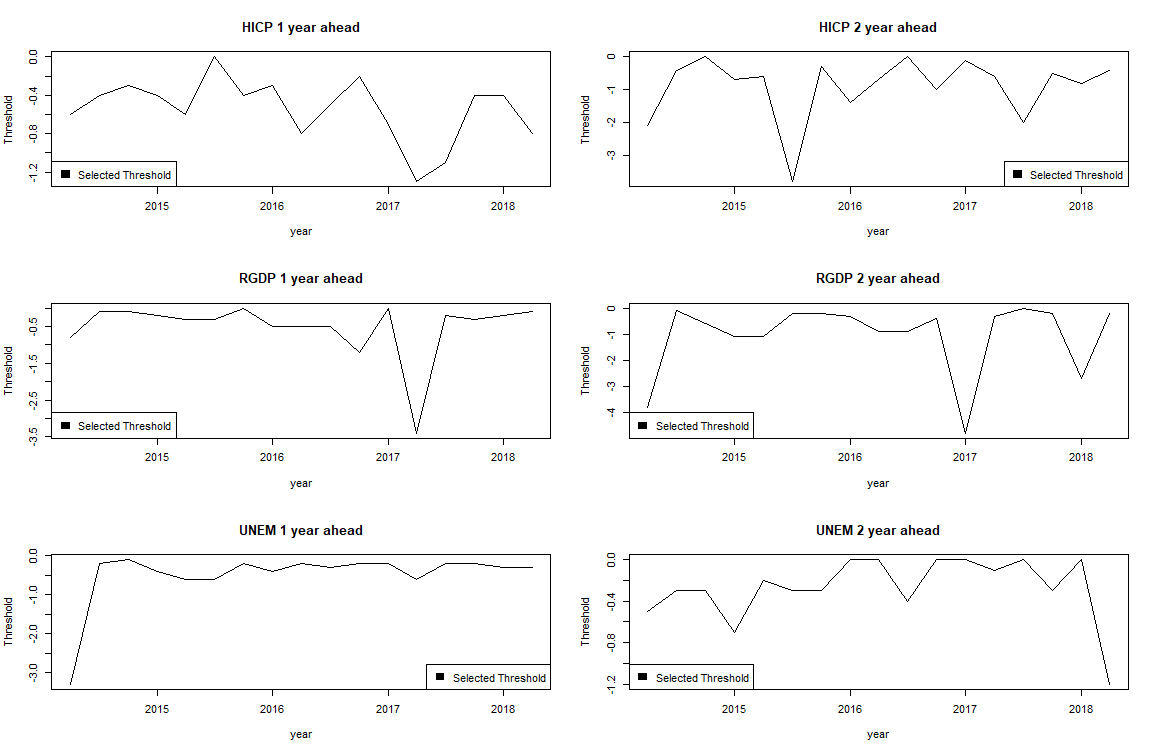
\includegraphics{./Images/Fluctuation.pdf}
	\caption{Truncation selection for different OOS period}\label{fig: fluctuation}
\end{figure}

\subsection{Bias weighting}\label{bias-weighting}

The bias weighting is an interesting case here. If the model in the bias estimation successfully estimates the predictable part and the unpredictable error, this can attribute to a better weight selection with additional information gained. Our approach to bias estimation is similar to \cite{Gibbs2017} but deviates in the variable used. We estimate the bias by
\begin{equation}
\label{eqn: bias estimation}
\epsilon_{i,t} = \alpha + \gamma_i y_{i,t} + \eta_{i,t},
\end{equation}
which we then produce the estimated future forecast bias by taking the expected value
\begin{equation}
E(\epsilon_{i,t+1}) = \alpha + \gamma_i y_{i,t+1}.
\end{equation}
\citeauthor{Gibbs2017} uses the true macroeconomic data, while we uses the forecast itself. Essentially they are interchangeable. Rewrite equation \ref{eqn: bias estimation} into
\begin{equation}
\begin{aligned}
\epsilon_{i,t} &= \frac{\alpha}{1+\gamma_i}+\frac{\gamma_i}{1+\gamma_i}y_t + \frac{1}{1+\gamma_i}\eta_{i,t}\\
&= \alpha^* + \gamma_i^* y_t + \eta_{i,t}^*,
\end{aligned} 
\end{equation}
and equation \ref{eqn: bias estimation} becomes the equation given by \citeauthor{Gibbs2017}.

Table \ref{tab: MSPE HICP bias}, \ref{tab: MSPE RGDP bias}, and \ref{tab: MSPE UNEM bias} shows the effect of truncation with bias-corrected weight. The estimation of bias increases the estimation error and therefore is another trade-off between estimation error and the bias. Only two out of six topics have a ratio below 1, considerably worse than without bias correction. The two topics are RGDP two years and UNEM one year, with a minimum of 0.83 and 0.56 respectively. For HICP with bias correction, the truncation performs best with the highest value. This is different from no-bias selection.

\begin{table}[!h]
	\centering
	\caption{Mean Squared Prediction Error (MSPE) of bias-corrected inflation with different truncated value. The MSPE of the truncated value is given in the ratio of truncation to equal weight. Larger than 1 means truncated is worse, whereas smaller than 1 means truncated weight helps in reducing MSPE.}
	\label{tab: MSPE HICP bias}
	\begin{tabular}{lcccc}
		\hline
		&                        \multicolumn{4}{c}{HICP}                         \\
		\cmidrule(lr){2-5}                              & \multicolumn{2}{c}{one year Horizon} & \multicolumn{2}{c}{two years Horizon} \\
		\cmidrule(lr){2-3} \cmidrule(lr){4-5}
		Threshold & MSPE Ratio & MAPE Ratio  & MSPE Ratio & MAPE Ratio  \\ \hline
		-$\infty$ & 2.7747 & 1.7760 & 1.6452 & 1.3735\\ 
		-5 & 2.7747 & 1.7760 & 1.6452 & 1.3735\\ 
		-4.5 & 2.7747 & 1.7760 & 1.6452 & 1.3735\\ 
		-4 & 2.7747 & 1.7760 & 1.6452 & 1.3735\\ 
		-3.5 & 2.7747 & 1.7760 & 1.6452 & 1.3735\\ 
		-3 & 2.7747 & 1.7760 & 1.5888 & 1.2976\\ 
		-2.5 & 2.7747 & 1.7760 & 1.6059 & 1.3276\\ 
		-2 & 2.7747 & 1.7760 & 1.5955 & 1.3064\\ 
		-1.5 & 2.7747 & 1.7760 & 1.5887 & 1.2871\\ 
		-1 & 2.6528 & 1.6894 & 1.1640 & 1.1141\\ 
		-0.5 & 1.7696 & 1.3260 & 1.0464 & 1.0365\\ 
		0 & 1.1118 & 1.0576 & 1.0221 & 1.0231\\ \hline
	\end{tabular}
\end{table}


RGDP shows similar results in one year, where truncation helps, but selecting 0 is the best performing one. On the other hand, RGDP two years shows that it can achieve an MSPE ratio of 0.83 with a truncation value of -1. The selection from MAPE ratio yields the same truncation. Comparing this to RGDP without bias correction, the bias-corrected performs worse in one year horizon, while performing better in two years horizon. The best truncation also changes to a different value, from -1.5 for one year horizon and 0 for two years horizon in no correction to 0 and -1 respectively.

\begin{table}[!h]
	\centering
	\caption{Mean Squared Prediction Error (MSPE) of bias-corrected economic growth with different truncated value. The MSPE of the truncated value is given in the ratio of truncation to equal weight. Larger than 1 means truncated is worse, whereas smaller than 1 means truncated weight helps in reducing MSPE.}
	\label{tab: MSPE RGDP bias}
	\begin{tabular}{lcccc}
		\hline
		&                        \multicolumn{4}{c}{RGDP}                         \\
		\cmidrule(lr){2-5}                              & \multicolumn{2}{c}{one year Horizon} & \multicolumn{2}{c}{two years Horizon} \\
		\cmidrule(lr){2-3} \cmidrule(lr){4-5}
		Threshold & MSPE Ratio & MAPE Ratio  & MSPE Ratio & MAPE Ratio  \\ \hline
		-$\infty$ & 3.3002 & 1.5457 & 1.0535 & 0.9458\\ 
		-5 & 1.7581 & 1.2626 & 1.1094 & 0.9846\\ 
		-4.5 & 1.7915 & 1.2894 & 1.1094 & 0.9846\\ 
		-4 & 1.7910 & 1.2888 & 1.1069 & 0.9833\\ 
		-3.5 & 1.8086 & 1.298 & 1.1079 & 0.9838\\ 
		-3 & 1.8101 & 1.2984 & 1.1076 & 0.9837\\ 
		-2.5 & 1.8118 & 1.3004 & 1.0691 & 0.9716\\ 
		-2 & 1.6089 & 1.3075 & 0.9950 & 0.9438\\ 
		-1.5 & 1.4604 & 1.2530 & 0.8630 & 0.8931\\ 
		-1 & 1.2764 & 1.1320 & 0.8275 & 0.8753\\ 
		-0.5 & 1.0758 & 1.0464 & 0.9437 & 0.9508\\ 
		0 & 1.0436 & 1.0264 & 0.9835 & 0.9892\\ \hline
	\end{tabular}
\end{table}


With UNEM one year as low as 0.56, UNEM achieved is a large improvement to the equal weight case. However, this effect does not show in the two years horizon. The two years horizon MSPE ratio increased to higher than equal weight.


\begin{table}[!h]
	\centering
	\caption{Mean Squared Prediction Error (MSPE) of bias-corrected unemployment with different truncated value. The MSPE of the truncated value is given in the ratio of truncation to equal weight. Larger than 1 means truncated is worse, whereas smaller than 1 means truncated weight helps in reducing MSPE.}
	\label{tab: MSPE UNEM bias}
	\begin{tabular}{lcccc}
		\hline
		&                        \multicolumn{4}{c}{UNEM}                         \\
		\cmidrule(lr){2-5}                              & \multicolumn{2}{c}{one year Horizon} & \multicolumn{2}{c}{two years Horizon} \\
		\cmidrule(lr){2-3} \cmidrule(lr){4-5}
		Threshold & MSPE Ratio & MAPE Ratio  & MSPE Ratio & MAPE Ratio  \\ \hline
		-$\infty$ & 3.7993 & 1.4829 & 21.2312 & 3.0358\\ 
		-5 & 3.7993 & 1.4829 & 2.5172 & 1.5149\\ 
		-4.5 & 3.7993 & 1.4829 & 2.5172 & 1.5149\\ 
		-4 & 3.7993 & 1.4829 & 2.5376 & 1.5293\\ 
		-3.5 & 3.7993 & 1.4829 & 2.5287 & 1.5246\\ 
		-3 & 3.3185 & 1.3959 & 2.3569 & 1.4439\\ 
		-2.5 & 2.3783 & 1.1662 & 2.3491 & 1.4493\\ 
		-2 & 0.9828 & 0.8032 & 2.3203 & 1.4382\\ 
		-1.5 & 0.7950 & 0.7275 & 1.6368 & 1.2530\\ 
		-1 & 0.5564 & 0.6864 & 1.3372 & 1.1226\\ 
		-0.5 & 0.7253 & 0.8155 & 1.1141 & 1.0643\\ 
		0 & 0.8736 & 0.9201 & 1.0327 & 1.0176\\ \hline
	\end{tabular}
\end{table}

Figure \ref{fig: Ratio bias} shows the MSPE ratio and MAPE ratio over the different threshold in higher granularity. HICP does not attend the minimum with a threshold up to 0 for both forecast horizon. The same conclusion also holds for RGDP one year and UNEM two years. On the other hand, RGDP two years has a large effect in truncation with bias-correction occurs, while performs badly without bias-correction. One reason for this is that the problem with RGDP is highly biasses over time, which cannot be corrected using cross-sectional truncation. UNEM one year is another macroeconomic topic that performs better with bias correction. We see from the plot that a large area is well below 0.7, relieving the problem of selecting precisely -0.5.


\begin{figure}[!h]
	\centering
	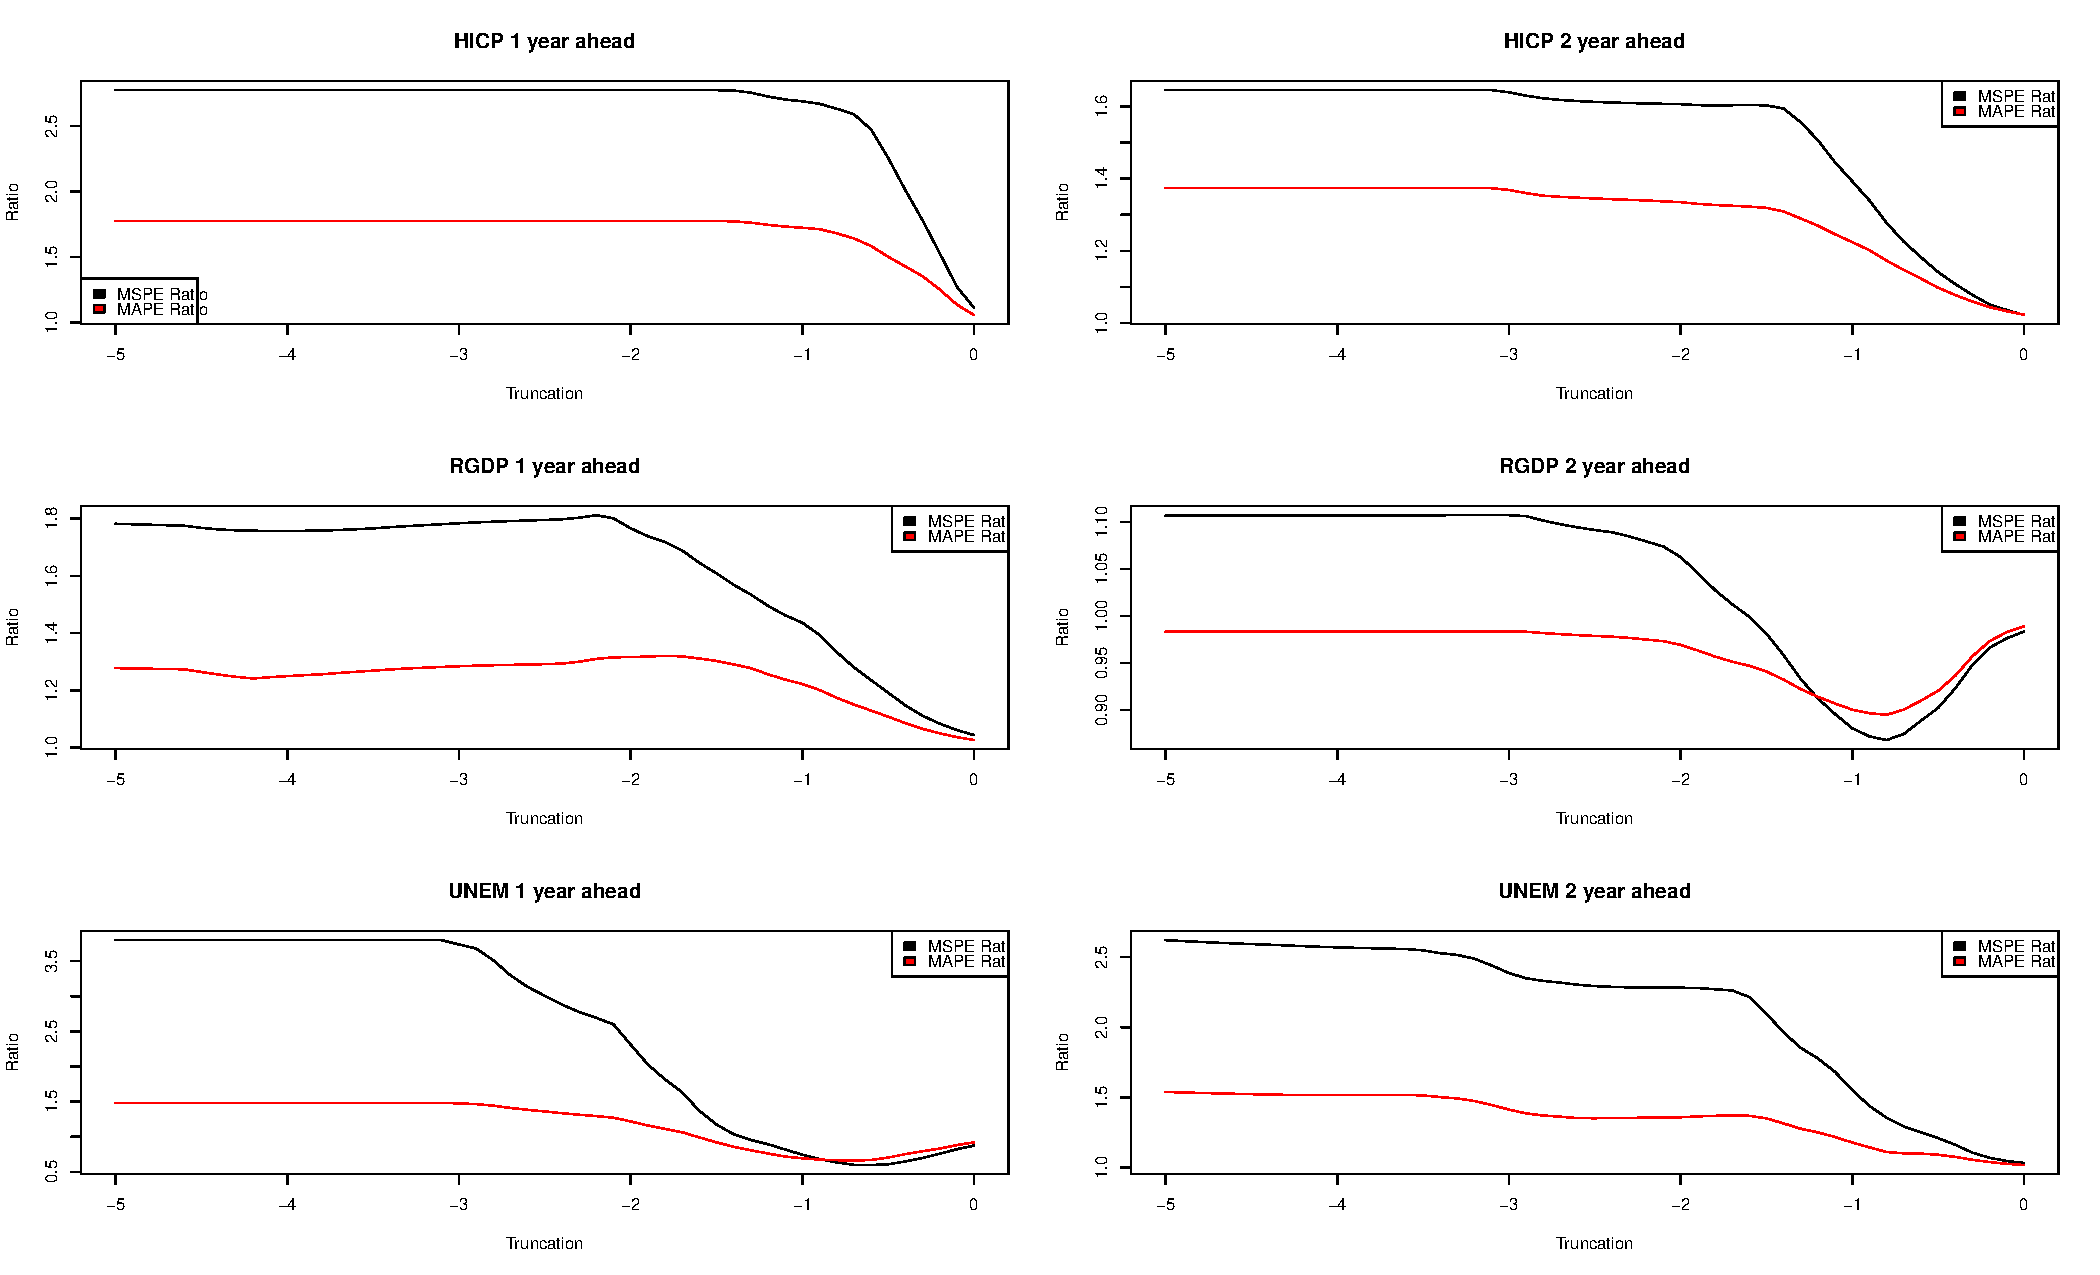
\includegraphics{./Images/Ratio_c_bias.pdf}
	\caption{MSPE Ratio for different macroeconomic topics with bias correction}\label{fig: Ratio bias}
\end{figure}


\begin{figure}[!h]
	\centering
	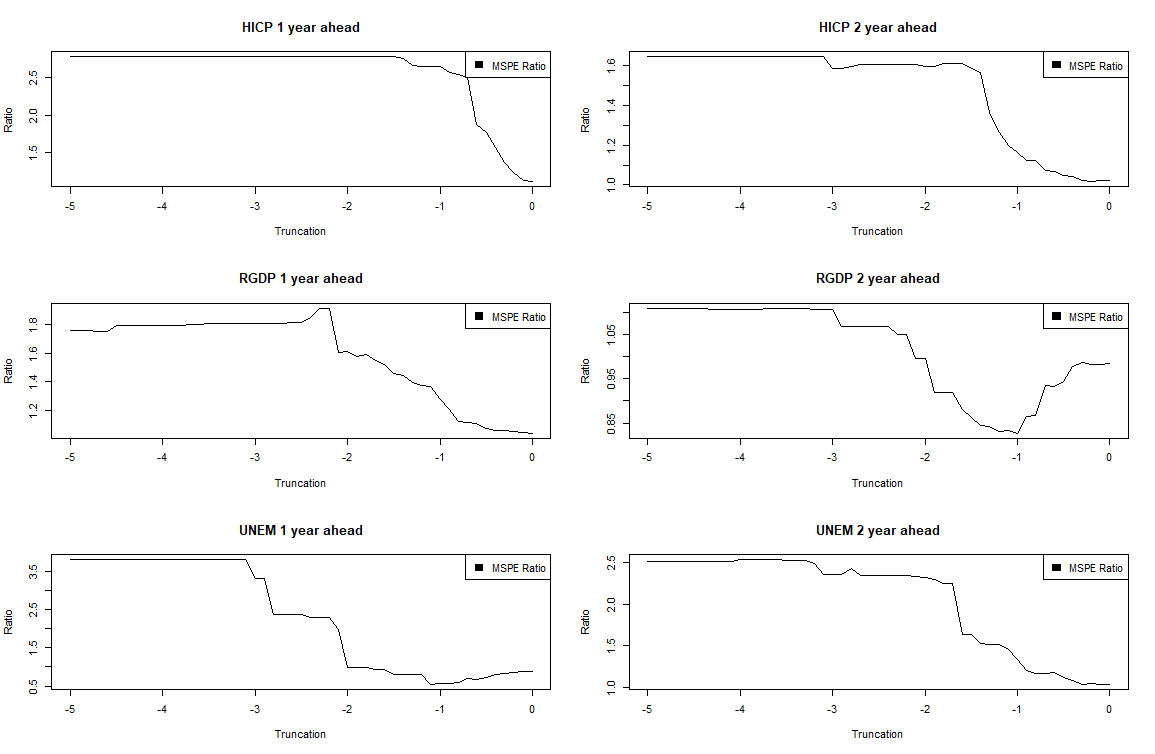
\includegraphics{./Images/Ratio Bias.pdf}
	\caption{MSPE Ratio for different macroeconomic topics with bias correction}\label{fig: Ratio bias}
\end{figure}


All in all, we observed the possibility to combine bias-correction and truncation. Some macroeconomic performs better with the only truncation, while some perform better with the addition of bias-correction. A possible explanation is that the truncation has effect in a different direction than the bias-correction. Truncation relies on the high correlation between different $y_i$, while bias-correction relies on the consistency and predictability of the forecast error in a univariate setting. This difference between the two approaches explains the different effect between series. If the predictability of the forecast error is small, such that predicting the forecast increases the MSE, adjusting the bias does not help. Of course, the truncation and bias-correction are not mutually independent. An increase in the correlation increases the similarity of the estimation error. In turn, the estimation errors do not cancel out but magnify. 



\subsection{Simulation}\label{simulation}
In this section, we show a different effect on the underlying model influences the MSPE. For simplicity, we select four true weights and change the data generating model regarding correlation and error variance. We start with the true weight as $w=(-0.5,0.3,0,1.2)'$, and proceed with the correlation matrix where all off-diagonals are the same value. Covariance matrix follows by setting all variance to 1. The error term is generated with a univariate random normal distribution, while the forecasts are generated by multivariate normal. We do not use biased forecast in this simulation. The simulation runs 10 observations per time for 2000 times for each correlation and error variance combination. Then the simulation takes the average of the MSPE.

In figure \ref{fig: simulation} different effects of correlation and error variance are shown. We select four different correlation, from 0.5 to 0.8, covering most of the correlation we observed in SPF. For the error variance, we show a range of selection from 0.4 to 0.9. Since the data variance is 1, the error variance quickly gives an idea on the fit of each forecast. 

From figure \ref{fig: simulation}, changes in the correlation and error variance does not influence the position where the MSPE drops or rises. Changes in error variance influence trivially on the level of MSPE. Higher error variance leads to higher MSPE. Changes in correlation show the location where the truncation effect converge to. For low correlation, 0.5 and 0.6, there is a distinct upward movement when truncation goes to 0 for all error variance. This forms the U-shape one expect when the bias increases. For high correlation, the effect of truncation does not increase the bias large enough, making the U-shape observable in only a few cases. Other cases with higher error variance show a continuous decline in MSPE. 

Referring back to section \ref{bias-weighting}, the changes in the shape can be accounted for the additional estimation error caused by the bias term. In figure \ref{fig: simulation}, it would be similar to plots of correlation 0.7 where error variance goes from 0.7 to 0.9.

For a U-shape to exist, e.g. equal weight is not the best, the correlation and error variance both plays an important role. Higher correlation only allows lower error when finding the optimal truncation parameter, while a lower correlation also allows higher error to exist.

\begin{figure}[!h]
	\centering
	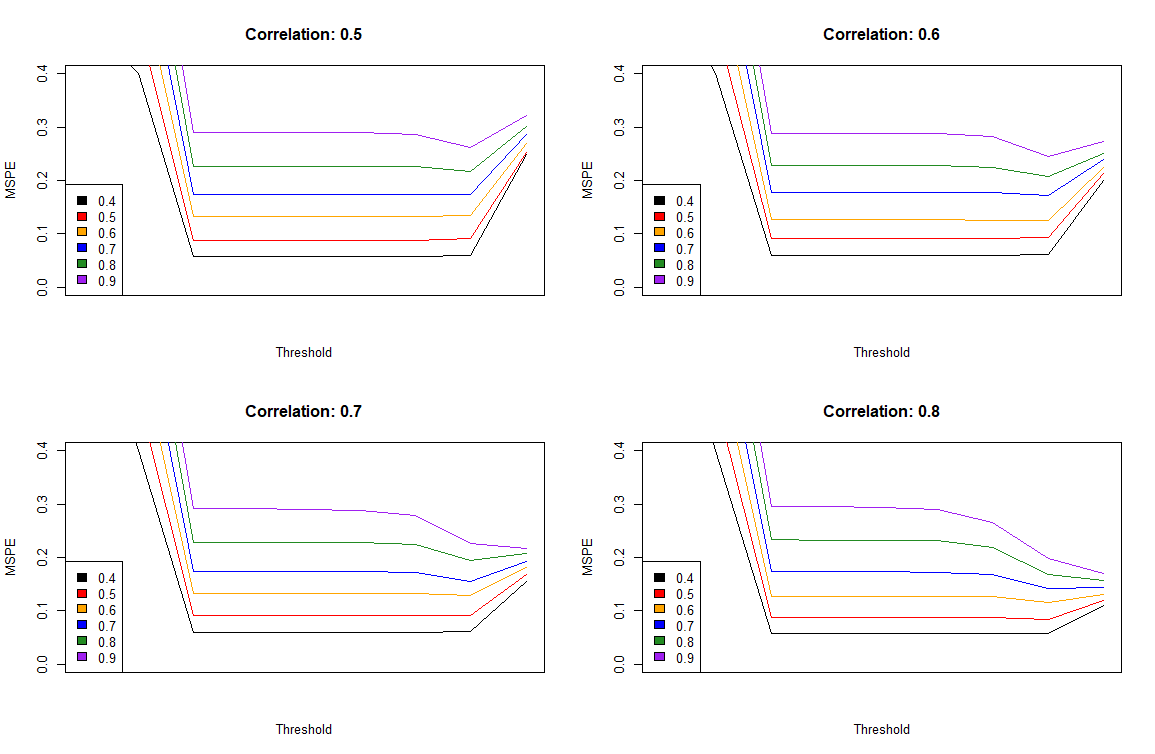
\includegraphics{./Images/Simulation.pdf}
	\caption{MSPE for different correlation and different error variance.}\label{fig: simulation}
\end{figure}

\section{Conclusion and discussion}\label{conclusion}
In this paper, we look into the possibility to use truncation to improve the forecast within the forecast combination. Simple weight derived with a deterministic weight assumption often shows bad empirical behaviour when compared to equal weight by arithmetic mean. Equal weight has a behaviour that the combined forecast cannot exceed the minimum or the maximum of all forecast. This limitation also holds for all weight selection method where the weight cannot be negative. 

Using truncation, five out of six macroeconomic topics have a positive effect on the mean squared prediction error (MSPE) and mean absolute prediction error (MAPE) for the European Central Bank's (ECB) survey of professional forecasters (SPF). SPF is a quarterly survey sent to the private sector to understand their view on inflation (HICP), economic growth (RGDP), and unemployment (UNEM) in the next one and two year. The survey forecasts have a strong correlation within the forecasters, which we show that the true value often lies outside of the minimum/maximum range. Additionally, the increase in the correlation leads to an increase in the negative weight. Therefore the relaxation of no negative weight helps in this aspect.

By truncation, we also set the weight below a certain threshold to 0, which removes the forecasts from the combination list. The results indicate a positive effect up to 30\% decrease in MSPE compared to equal weight. This is positive news considering the amount of forecaster is relatively large compared to the sample size. With up to 120 forecasters and 60 observations, the weight estimation contains a large amount of estimation noise. This gives the estimated weight a wide variation, with a minimum of -21.79 and maximum of 16.34. On the other hand, the weights calculated by equal weight method are around 0.01.

The effect of truncation comes into play for optimal threshold selection on the underlying truncation parameter. The decrease can go to as low as 12\% and 30\% in MSPE. Optimal threshold provides room for variation in parameter over time contrary to situations where parameters remain constant. This leads to a performance increase for RGDP with two years forecast horizon. Improvement in MAPE and MSPE is noted for all 6 microeconomic instances when the comparison is made for all equal weight. A majority of the parameters are under -1.5 for the chosen truncation. Of course, this is well under the initial -21.79. Variation is limited by setting the parameter under -1.5 thus reducing the estimation error and variance. 

Looking further into the weight selection, it is possible that the characteristic of SPF is dominated by a consistent bias over a certain forecaster. An example would be a case where the forecaster undervalues the growth and the decline, resulting in a forecast closer to 0 than the true value. Therefore we construct the bias correcting forecast weight and applies the truncation analysis on the corrected weight. The result is a mixed bag of good and bad news. Four out of six macroeconomic topics are worse than equal weight, while without bias correction, we have only 1 truncation weight that is under-performing. There are still declines in the test statistics compared to the non-truncated ones. On the positive news, bias-correction improves the only macro topic that does not outperform equal weight without bias-correction. The MSPE decreases up to 17\% compared with equal weight and MAPE up to 12 \%. Another positive news is an additional decrease of 13\% in UNEM one year ahead. The difference with and without bias correction could be in the direction of the changes in the weight. Truncation tries to extend the forecast upon the range by using negative weight, while bias-correction tries to identify the consistent bias within each forecaster.

We also study the different effect of correlation and estimation uncertainty on the shape of the MSPE. Correlation and estimation uncertainty both play important intertwined roles in the truncation. Higher correlation only allows lower error when finding the optimal truncation parameter, while a lower correlation also allows higher error to exist. Since estimation uncertainty and correlation can be known before applying truncation, the selection of best truncation using that information is a possible future research topic.

We list a few other points in this paper that require further research. All analytic derivations are done in two forecasts scenarios, which can be extended to the multivariate setting. RGDP two years ahead shows an unexpected shape of MSPE, with the reason for this shape unclear. Knowing the reason for spikes in the truncation selection is helpful as this can help in limiting variation — a combination of other techniques like shrinkage on the covariance to improve the estimates. Additionally, use the threshold value instead of 0 to the truncation can also change the effect of the method.

All in all, we demonstrate the ability to improve upon equal weight by truncation. The requirements for the improvement lies in the correlation and forecast uncertainty. When the conditions are met, for example, the SPF data, equal weight is no longer the prime choice in the forecast combination. 

\newpage

\bibliographystyle{apalike}
\bibliography{shortbib}

\end{document}


